\documentclass[12pt, a4paper, twoside, openright]{report}
\input{preamble.tex}

\AtBeginDocument{\RenewCommandCopy\qty\SI}

\title{\textbf{Fisher-Kolmogorov}\\Equation for neurodegenerative diseases}
\author{Lorenzo Esposito 10765981, Francesco Grassi 10841139, \\Giorgio Venezia 10807335}
\date{\today}


\begin{document}

\begin{textblock*}{\textwidth}(2.98cm,1.5cm)
  \begin{center}
    \maketitle
    Version 1.1.0
  \end{center}
\end{textblock*}


\blankpage

% ============== Indice ============== %
\tableofcontents
\afterpage{\blankpage}
\newpage
\pagenumbering{arabic}

\chapter{Introduction}

Neurodegenerative diseases such as Alzheimer's, Parkinson's, and ALS involve progressive neuronal death caused by misfolded proteins that spread through brain tissue. These diseases follow a prion-like mechanism in which pathogenic proteins convert normal proteins into toxic aggregates, creating cascading propagation across neural networks.

Mathematical modeling uses reaction-diffusion equations to capture this spreading process. The models treat protein aggregation as a non-linear reaction coupled with anisotropic diffusion through brain tissue, reducing the biology mechanism to equations governing protein concentration dynamics in space and time.

This project implements a physics-based reaction-diffusion model combining the Fisher-Kolmogorov equation with directional diffusion terms inspired by the framework presented in the article \cite{WEICKENMEIER2019264}. The model simulates growth and diffusion in terms of concentration of misfolded protein.

If these models are accurate, they can predict disease progression patterns, identify vulnerable brain regions, and inform therapeutic strategies targeting early-stage protein aggregation before irreversible neuronal damage occurs.



\chapter{Problem model definition}
The mathematical formulation of the problem is given by
\begin{equation} \label{fisher-kolmogorov}
  \begin{cases}
    \displaystyle
    \frac{\partial c}{\partial t} - \nabla \cdot (D \cdot \nabla c) - \alpha c(1-c) = 0 & \textrm{in} \ \Omega \times \left[0,T\right],          \\

    \displaystyle
    D \cdot \nabla c \cdot \vec{n} = 0                                                  & \textrm{in} \ \partial \Omega \times \left[0,T\right], \\

    \displaystyle
    c(t=0)=c_{0}                                                                        & \textrm{in} \ \Omega.                                  \\
  \end{cases}
\end{equation}
where $c : \left[0,T\right] \times \Omega \to \mathbb{R}$ is the unknown function,
$D \in \mathbb{R}^{n \times n}$ is the diffusion tensor,
$\alpha \in \mathbb{R}^{+}$ is a given parameter,
$\Omega \subset \mathbb{R}^n$ is a bounded domain, and
$\vec{n}$ denotes the outward unit normal vector on $\partial \Omega$.

\section{Kinetics of prion-like spreading}
To describe the fundamental mechanism behind prion-like
spreading, the article \cite{WEICKENMEIER2019264} presents a
simplified kinetic model, which distinguishes between two states
of a protein: the natural healthy form $p$ and the misfolded,
pathogenic form $\tilde{p}$. The misfolded proteins propagate
through the brain by converting healthy proteins into their
misfolded form, in an autocatalytic fashion.

The model considers the following kinetic processes:
\begin{itemize}
  \item \textbf{Recruitment and conversion:} Healthy proteins bind to misfolded proteins and adopt the misfolded state at a rate $k_{12}$:
        \[
          p + \tilde{p} \xrightarrow{k_{12}} \tilde{p}+\tilde{p}.
        \]
        More explicitly, this overall reaction is the result of a chain of steps:
        \[
          p + \tilde{p} \;\to\; p\tilde{p} \;\to\; \tilde{p}\tilde{p} \;\to\; \tilde{p} + \tilde{p},
        \]
        where the first step corresponds to recruitment, the second to conversion, and the last to fragmentation of the misfolded dimer.

  \item \textbf{Fragmentation:} Misfolded proteins can fragment to generate new infectious seeds (although this process is not explicitly retained in the final formulation).

  \item \textbf{Production and clearance:} Healthy proteins are continuously produced at a constant rate $k_0$ and cleared at rate $k_1$, while misfolded proteins are cleared at a separate rate $\tilde{k}_1$.

  \item \textbf{Diffusion:} Both types of proteins diffuse in the surrounding medium, with diffusion tensors $D_p$ and $D_{\tilde{p}}$.
\end{itemize}

The model leads to a system of coupled PDEs governing the evolution of the concentrations of the two protein types:
\begin{align}
  \pdv{p}{t}         & = \Div(D_p \nabla p) + k_0 - k_1 p - k_{12}p\tilde{p},                             \\
  \pdv{\tilde{p}}{t} & = \Div(D_{\tilde{p}} \nabla \tilde{p}) - \tilde{k}_1 \tilde{p} + k_{12}p\tilde{p}.
\end{align}

To simplify the system, \cite{WEICKENMEIER2019264} assumes that the concentration of healthy protein is significantly higher than that of the misfolded form (i.e., $p \gg \tilde{p}$), allowing a quasi-steady-state approximation for $p$. Under this assumption, the healthy protein concentration is approximated as
\begin{equation}
  p \approx \frac{k_0}{k_1 + k_{12}\tilde{p}}.
\end{equation}

Expanding this expression in a Taylor series around $\tilde{p}=0$ and substituting it into the equation for $\tilde{p}$ yields a nonlinear reaction–diffusion equation.

To further simplify the model, a normalized concentration is introduced for misfolded proteins:
\begin{equation}
  c = \frac{\tilde{p}}{\tilde{p}_{\max}}, \qquad 0 \leq c \leq 1.
\end{equation}

This leads to a logistic-type equation:
\begin{equation}
  \pdv{c}{t} = \Div(D \nabla c) + \alpha c (1 - c),
\end{equation}
where $D = D_{\tilde{p}}$ is the diffusion tensor and $\alpha$ is the effective growth rate defined as
\begin{equation} \label{alpha_def}
  \alpha = \frac{k_{12} k_0}{k_1} - \tilde{k}_1.
\end{equation}

\autoref{alpha_def} captures the key dynamics of prion-like propagation: the diffusion of misfolded proteins and their growth due to the conversion of healthy proteins. The growth rate $\alpha$ increases with the conversion rate $k_{12}$ and the equilibrium healthy protein concentration $p_0 = k_0/k_1$, and decreases with the clearance rate of misfolded proteins $\tilde{k}_1$.

\subsection{Diffusion tensor} \label{diff_term_math}

If $\Omega \subset \mathbb{R}^3$ the diffusion term is represented by a tensor \(\mathbf{D}\), which accounts for both isotropic and anisotropic transport of misfolded proteins:
\begin{equation}
  \mathbf{D} = d^{\mathrm{ext}} \mathbf{I} + d^{\mathrm{axn}} \, \mathbf{n} \otimes \mathbf{n}.
\end{equation}
Here, \(d^{\mathrm{ext}}\) denotes the isotropic extracellular diffusion, while \(d^{\mathrm{axn}}\) represents anisotropic transport along axonal fibers. The unit vector \(\mathbf{n}\) indicates the local fiber direction.

Else, if $\Omega \subset \mathbb{R}$, the diffusion term reduces to a scalar coefficient:
\begin{equation}
  D = d \in \mathbb{R},
\end{equation}
since anisotropic effects cannot be represented in a single spatial dimension.



\section{Weak formulation}
As for most partial differential equations, the first step is to construct the weak formulation.
\begin{enumerate}
  \item To derive the weak formulation, we introduce the Hilbert space
        \[
          H^1(\Omega) = \left\{ v \in L^2(\Omega) \, : \, \nabla v \in \left[L^2(\Omega)\right]^d \right\}.
        \]
        It is required that $c \in H^1(\Omega)$ in order to be a solution of \autoref{fisher-kolmogorov}.

  \item For a function $c \in H^1(\Omega)$ to be a solution of \autoref{fisher-kolmogorov}, it is required that $\forall v \in H^1(\Omega)$:
        \begin{equation}
          \label{test_func}
          \int_{\Omega} \pdv{c}{t} \, v \, \mathrm{d}\mathbf{x}
          - \int_{\Omega} \nabla \cdot (D \nabla c) \, v \, \mathrm{d}\mathbf{x}
          - \int_{\Omega} \alpha c(1-c) \, v \, \mathrm{d}\mathbf{x} = 0.
        \end{equation}

  \item By integrating by parts the second term, $-\int_{\Omega} \nabla \cdot (D \nabla c) \, v \, \mathrm{d}\mathbf{x}$, we obtain:
        \begin{equation}
          \label{integrate_by_parts}
          - \int_{\Omega} \nabla \cdot (D \nabla c) \, v \, \mathrm{d}\mathbf{x}
          = \int_{\Omega} D \nabla c \cdot \nabla v \, \mathrm{d}\mathbf{x}
          - \int_{\partial \Omega} (D \nabla c \cdot \vec{n}) \, v \, \mathrm{d}s.
        \end{equation}
        The boundary term $\int_{\partial \Omega} (D \nabla c \cdot \vec{n}) \, v \, \mathrm{d}s$ vanishes due to the second condition in \autoref{fisher-kolmogorov}. Substituting into \autoref{test_func}, we obtain the weak formulation of \autoref{fisher-kolmogorov}:
        \begin{equation}
          \label{weak_formulation}
          \int_{\Omega} \pdv{c}{t} \, v \, \mathrm{d}\mathbf{x}
          + \int_{\Omega} D \nabla c \cdot \nabla v \, \mathrm{d}\mathbf{x}
          - \int_{\Omega} \alpha c(1-c) \, v \, \mathrm{d}\mathbf{x} = 0.
        \end{equation}
\end{enumerate}

\section{Time discretization}
Since \autoref{weak_formulation} contains the term $\int_{\Omega} \pdv{c}{t} \, v \, \mathrm{d}\mathbf{x}$, it is necessary to discretize the time derivative.
We choose the Backward Euler method (BEM) for two reasons. First, it is unconditionally stable, since it can be regarded as a special case of the $\theta$-method with $\theta=1$, where unconditional stability holds for $\theta \geq 1/2$. In contrast, for example, the Forward Euler method is not unconditionally stable. The second reason is that BEM is less computationally expensive than other unconditionally stable methods, such as the Midpoint method.

We consider the time interval $(0, T]$, where $T$ is the final simulation time, and divide it into $N$ equal subintervals of length $\Delta t = T/N$. For each time step $t^{n+1}$, the time derivative can be approximated as
\[
  \left. \pdv{c}{t} \right|_{t^{n+1}} \approx \frac{c^{n+1} - c^n}{\Delta t},
\]
We define the trial and test space as $V = H^1(\Omega)$ which leads to the fully discrete weak formulation:
\begin{quote}
  \textit{Find $c^{n+1} \in V$ such that for all $v \in V$ it holds that}
  \begin{equation}
    \label{time_discretization}
    \int_{\Omega} \frac{c^{n+1} - c^n}{\Delta t} \, v \, \mathrm{d}\mathbf{x}
    + \int_{\Omega} D \nabla c^{n+1} \cdot \nabla v \, \mathrm{d}\mathbf{x}
    - \int_{\Omega} \alpha c^{n+1}(1-c^{n+1}) \, v \, \mathrm{d}\mathbf{x} = 0.
  \end{equation}
\end{quote}


\section{Linearization}

It is still not possible to utilize \autoref{time_discretization} for the numerical solution because it contains a nonlinear term, namely
\[
  - \int_{\Omega} \alpha c^{n+1}(1-c^{n+1}) \, v \, dx .
\]
To solve the problem, we need to use a linearized form of \autoref{time_discretization}. This can be done using the Fréchet derivative.

For a given functional $G : V \rightarrow \mathbb{R}$, the Fréchet derivative at a point $u \in H^1(\Omega)$ is a linear operator $A(u) = \frac{dG}{du}: V \rightarrow \mathbb{R}$ such that
\[
  \lim_{\|d\| \to 0} \frac{\left| G(u + d) - G(u) - A(u)d \right|}{\|d\|} = 0 .
\]

We now define the nonlinear residual:
\begin{equation}
  \label{residual}
  \begin{aligned}
    R(c^{n+1} + \delta, v) =\; & \int_{\Omega} \frac{c^{n+1} + \delta - c^n}{\Delta t} \, v \, dx
    + \int_{\Omega} D \nabla (c^{n+1} + \delta) \cdot \nabla v \, dx                                          \\
                               & - \int_{\Omega} \alpha (c^{n+1} + \delta)(1 - c^{n+1} - \delta) \, v \, dx .
  \end{aligned}
\end{equation}

Subtracting $R(c^{n+1}, v)$, we obtain:
\begin{equation}
  \label{difference_residual}
  \begin{aligned}
    R(c^{n+1} + \delta, v) - R(c^{n+1}, v) =\; &
    \int_{\Omega} \frac{\delta}{\Delta t} \, v \, dx
    + \int_{\Omega} D \nabla \delta \cdot \nabla v \, dx                                                                         \\
                                               & - \int_{\Omega} \alpha \bigl( \delta (1 - 2c^{n+1}) - \delta^2 \bigr) v \, dx .
  \end{aligned}
\end{equation}

Approximating $\delta^2$ as a higher-order small term, we arrive at:
\begin{equation}
  \label{delta_residual}
  \begin{aligned}
    R(c^{n+1} + \delta, v) - R(c^{n+1}, v) =\; &
    \int_{\Omega} \frac{\delta}{\Delta t} \, v \, dx
    + \int_{\Omega} D \nabla \delta \cdot \nabla v \, dx                                                  \\
                                               & - \int_{\Omega} \alpha \delta (1  - 2c^{n+1}) \, v \, dx
    + \mathcal{O}(\delta^2).
  \end{aligned}
\end{equation}

The right-hand side of \autoref{delta_residual}, up to $\mathcal{O}(\delta^2)$, corresponds to the action of the Fréchet derivative:
\[
  \frac{dR}{dc}(c^{n+1})(\delta, v) = a(c^{n+1})(\delta, v).
\]

Thus, solving \autoref{time_discretization} is equivalent to finding $c^{n+1} \in H^1(\Omega)$ such that
\[
  R(c^{n+1}, v) = 0, \quad \forall v \in H^1(\Omega).
\]

To this end, we employ Newton's method


\begin{algorithmic}
  \State Given an initial guess $c^{(0)}$,
  \While{$k = 1,2,\dots,N$ \textbf{ and not converged}}
  \State \textbf{find} $\delta^{(k)}$ such that
  \[
    a(c_k^{n+1})(\delta^{(k)}, v) = -R(c_k^{n+1}, v), \quad \forall v \in H^1(\Omega),
  \]
  \State and update
  \[
    c^{(k+1)} = c_k^{n+1} + \delta^{(k)}.
  \]
  \EndWhile
\end{algorithmic}

The problem
\[
  a(c_k^{n+1})(\delta^{(k)}, v) = -R(c_k^{n+1}, v)
\]
is a linear variational problem, which can be solved using the finite element method.


\section{Finite element setting and final assembly}

After deriving a linear differential form of the original problem in \autoref{fisher-kolmogorov} in the form
\[
  a(c_k^{n+1})(\delta^{(k)}, v) = -R(c_k^{n+1}, v),
\]
we discretize the problem in space using the Galerkin finite element method.
To this end, we consider a finite-dimensional vector space \(V_h \subset H^1(\Omega)\) with dimension \(N_h\).
Our goal is to find \(\delta_h^{(k)}\) such that
\[
  a(c_h^{(k)})(\delta^{(k)}, v_h) = -R(c_h^{(k)}, v_h) \qquad \forall v_h \in V_h.
\]

We introduce the basis of \(V_h\), denoted by \(\{\phi_j\}_{j=1}^{N_h}\), and expand the unknowns as
\[
  c_h^{(k)}(\mathbf{x}) = \sum_{j=1}^{N_h} c_j^{(k)} \phi_j(\mathbf{x}),
  \qquad
  \delta^{(k)}(\mathbf{x}) = \sum_{j=1}^{N_h} \delta_j^{(k)} \phi_j(\mathbf{x}).
\]
Substituting these expressions into the weak problem and choosing the test functions as \(v_h=\phi_i\) gives
\begin{equation}
  a \!\left( \sum_{j=1}^{N_h} c_j^{(k)} \phi_j(\mathbf{x}) \right)\!\!\left(\sum_{j=1}^{N_h} \delta_j^{(k)} \phi_j, \phi_i \right)
  = -R \!\left( \sum_{j=1}^{N_h} c_j^{(k)} \phi_j(\mathbf{x}), \phi_i \right).
\end{equation}

After straightforward computation, the following linear system is obtained:
\begin{equation}
  \label{linear_system}
  \left( \frac{M}{\Delta t} + K - J(c_k^{n+1}) \right)\delta^{(k)}
  = -M \frac{c_k^{n+1} - c^{n}}{\Delta t} - K c_k^{n+1} + N(c_k^{n+1}),
\end{equation}
where:
\begin{itemize}
  \item \(\delta^{(k)}\) is the vector of unknown coefficients at Newton iteration \(k\);
  \item \(c_k^{n+1}\) is the current approximation of the concentration at time step \(n+1\);
  \item \(c^{n}\) is the concentration computed at the previous time step \(n\);
  \item \(M = (m_{ij}), \quad m_{ij} = \int_{\Omega} \phi_i \phi_j \, \mathrm{d}\mathbf{x}\) is the mass matrix;
  \item \(K = (k_{ij}), \quad k_{ij} = \int_{\Omega} D \nabla \phi_i \cdot \nabla \phi_j \, \mathrm{d}\mathbf{x}\) is the stiffness matrix;
  \item \(J(c_k^{n+1}) = (j_{ij}), \quad j_{ij} = \int_{\Omega} \alpha (1 - 2c_k^{n+1}) \phi_i \phi_j \, \mathrm{d}\mathbf{x}\) is the Jacobian of the reaction term;
  \item \(N(c_k^{n+1}) = (n_i), \quad n_i = \int_{\Omega} \alpha \, c_k^{n+1}(1 - c_k^{n+1}) \phi_i \, \mathrm{d}\mathbf{x}\) is the nonlinear reaction vector.
\end{itemize}

For clarity, we introduce the shorthand notation
\[
  LHS = \frac{M}{\Delta t} + K - J(c_k^{n+1}),
  \qquad
  RHS = -M \frac{c_k^{n+1} - c^{n}}{\Delta t} - K c_k^{n+1} + N(c_k^{n+1}).
\]

At each time step \(n+1\), the Newton method is applied to solve for \(\delta^{(k)}\) by solving the linear system in \autoref{linear_system}.
The increment \(\delta^{(k)}\) is then used to update the solution.
At every iteration of the Newton method, both the matrix \(LHS\) and the vector \(RHS\) are recomputed using the current approximation of the solution \(c_k^{n+1}\).



\chapter{Set up and computation}
The problem has been solved using \verb|C++| combining \verb|deal.ii| library and \verb|MPI| for the purpose of parallelization.

\section{1D and 3D: Key aspects}
The problem was initially solved in 1D as a proof of concept and to check feasibility, then scaled to 3D.
\subsection{The mesh}
The mesh used for 3D computation is read from an external \verb|.msh| file provided by the original author of the article \cite{WEICKENMEIER2019264}.
The implementation distinguishes between different brain tissue types through material IDs, with the code specifically tracking Grey Matter (material ID 1) and White Matter(material ID 2). A material mapping system associates each cell with its corresponding tissue type, enabling tissue-specific parameter assignment.

In 1D, the mesh is simply an interval $[0, l] \in \mathbb{R}$ divided into $N$ equal subintervals. For our computation, we have chosen $l=2$ and $N=200$.
\subsection{Diffusion Term}

As mentioned in \autoref{diff_term_math}, the diffusion term differs between the 1D and 3D formulations.

In the 3D formulation, the diffusion term is represented by a tensor \(\mathbf{D}\) that depends on the fiber direction \(\mathbf{n}\). The fiber direction can be defined according to different anatomical orientation models:
\begin{itemize}
  \item \textbf{Circumferential model:} fibers follow a path tangent to the cortical layers, forming circumferential rings.
  \item \textbf{Radial model:} fibers are oriented radially from the center of the brain outward toward the cortical surface.
  \item \textbf{Axonal model:} fibers are oriented along the principal direction of neural axons. In this case, diffusion in white matter follows the circumferential model, while in gray matter it follows the radial model, as shown in \cite{WEICKENMEIER2019264}.
\end{itemize}

These models allow the diffusion tensor to capture anisotropic spreading of misfolded proteins along specific tissue structures.

In the 1D simplification, the diffusion term reduces to a scalar coefficient:
\[
  D = d \in \mathbb{R},
\]
since anisotropic effects cannot be represented in a single spatial dimension.


\subsection{Similarity}
The methods used to solve equation had to be keeped unchanged, indeed the core structure of the algorithm stays unaltered:
\begin{itemize}
  \item Newton's method to solve nonlinear systems.
  \item Time-stepping stucture with backward Euler discretization.
  \item GMRES with preconditioner as linear solver.
\end{itemize}
\subsection{Differences}
\begin{itemize}
  \item 1D implementation uses a less complex and uniform mesh built with
        \[
          \verb|subdivided_hyper_cube()|.
        \]
        while 3D implementation reads the mesh directly from the proper file.

  \item In 1D the diffusion coefficient is just a scalar:
        \[
          \texttt{const double diffusion\_coefficient\_loc = diffusion\_coefficient.value();}
        \]
        while in 3D we model an anisotropic diffusion with tensor formulation:
        \[
          \texttt{const Tensor<2, dim> D = d\_ext\_matrix + d\_axn\_loc * normal\_matrix;}
        \]

  \item In 1D we assume uniform material properties throughout the domain, while the 3D program handles multiple brain tissue types (grey matter, white matter) through a gradient of $\alpha$.
\end{itemize}


\subsection{Parameters}\label{parameters}

The choice of the parameters is crucial for convergence, especially for 3D simulations. In this study, the inputs and parameters of the problem are:

\begin{enumerate}
  \item \(T\): final time of the simulation.
  \item \(\Delta t\): time step used for time discretization.
  \item Mesh: a 3D discretized representation of the domain in \(\mathbb{R}^3\).
  \item Degree: the polynomial degree of the finite elements used in the finite element method.
  \item \(d^{\mathrm{ext}}\): isotropic extracellular diffusion coefficient.
  \item \(d^{\mathrm{axn}}\): anisotropic axonal transport coefficient along fiber directions.
  \item Diffusion type: defines the orientation of misfolded protein transport. It can be:
        \begin{itemize}
          \item Axonal
          \item Circumferential
          \item Radial
        \end{itemize}
        These types of diffusion are also considered in \cite{WEICKENMEIER2019264}.
  \item \(\alpha\): growth rate of misfolded protein concentration.
  \item Initial seed: initial non-zero concentration.
  \item Seed region: subdomain in which the initial concentration is equal to the initial seed. In 3D simulations, a point \(x_0\) is provided, and the program constructs a spherical region centered at \(x_0\).
\end{enumerate}

\section{Implementation}
\subsection{Implementation in 1D}
To verify the correctness of our approach, we implemented a 1D solver following the methodology described in \cite{WEICKENMEIER2019264} and compared the results. In this case, the computational domain is the interval \([0,2] \subset \mathbb{R}\). The diffusion term \(D\) reduces to a scalar parameter \(d\), and the initial seed region consists of a single point at the center of the domain (\(x = 0\)).

The mesh is created over the interval with \(N = 200\) elements and polynomial degree equal to 1. After initializing all necessary objects, as done in the laboratory sessions, the method \texttt{solve()} executes the time-stepping procedure, computing the solution at each time step and writing the output to a \verb|.vtu| file.

The method \texttt{solve()} internally calls \texttt{solve\_newton()}, which performs Newton iterations to solve the nonlinear system. For each iteration, the system is linearized around the current solution by invoking \texttt{assemble\_system()}, and the resulting linear system is solved using \texttt{solve\_linear\_system()}. This process repeats until the norm of the residual vector falls below a fixed threshold, set to \(10^{-6}\) in our code.

\texttt{assemble\_system()} follows the same structure used in the laboratory exercises to compute the $LHS$ matrix and the $RHS$ vector. These terms represent the linearized versions of the original system, obtained using the values of the current and previous solutions along with the relevant parameters.

Since homogeneous Neumann boundary conditions are applied and Dirichlet conditions are absent, there is no need to handle boundary conditions explicitly.

\texttt{solve\_linear\_system()} assumes that the $LHS$ matrix and $RHS$ vector are correctly assembled. We use the Generalized Minimal Residual Method (GMRES) to solve the resulting linear system, and the SSOR preconditioner is applied to accelerate convergence.

\subsection{Implementation in 3D}

The primary differences in the 3D solver include the use of parallelization, the application of different parameters (as described in \autoref{parameters}), and the presence of two distinct material regions.

\subsubsection{Parallelization}

The 3D solver involves a substantially higher computational cost due to the large number of nodes in 3D meshes and the nonlinear nature of the problem. To make the computation feasible, parallelization is employed using Trilinos with MPI. The mesh is partitioned across multiple processes, with each process handling its assigned degrees of freedom and communicating with neighboring partitions at the boundaries. This domain decomposition allows the workload to be distributed efficiently across processes.

\subsubsection{Parameters representation}

\begin{itemize}
  \item \textbf{Mesh}: as described in \autoref{parameters}, the mesh is imported from an external \verb|.msh| file. Each element in the file includes a material ID, which can be 1 for Grey Matter or 2 for White Matter.
  
  \item \textbf{Piecewise function}: following \cite{WEICKENMEIER2019264}, the parameters \(d^{\mathrm{axn}}\), \(d^{\mathrm{ext}}\), and \(\alpha\) are assumed to be piecewise constant with respect to the material ID. This is implemented using a \verb|std::map<unsigned int, double>|, where each entry represents the value for a specific material ID (first entry for Grey Matter, second for White Matter). In the solver, the function \verb|virtual double value()| takes an additional argument \verb|const unsigned int component| to select the material ID corresponding to the point being evaluated. The \verb|component| value must be 1 or 2 to distinguish between Grey and White Matter.

  \item \textbf{Initial seed}: the initial seed region is computed as the intersection of a spherical region centered at the given seed point with the computational mesh.
\end{itemize}

In the 3D implementation, the SSOR preconditioner used in 1D was replaced by an ILU preconditioner due to better convergence behavior in the higher-dimensional problem.

\chapter{Performance evaluation}
The only case worth evaluating is the 3D implementation, as the 1D solver serves only as a proof of concept. In this section, we analyze the performance of the 3D solver in terms of scalability.

The results presented here are obtained using the parameter set from the first case in \cite{WEICKENMEIER2019264}:

\begin{itemize}
  \item \(T = \SI{20}{\year}\)
  \item \(\Delta t = \SI{0.1}{\year}\)
  \item \(d^{\mathrm{ext}} = [\SI[per-mode = symbol]{1.5}{\centi\meter\squared\per\year}, \SI[per-mode = symbol]{1.5}{\centi\meter\squared\per\year}]\)
  \item \(d^{\mathrm{axn}} = [\SI[per-mode = symbol]{0.0}{\centi\meter\squared\per\year}, \SI[per-mode = symbol]{3.0}{\centi\meter\squared\per\year}]\)
  \item \(\alpha = [\SI[per-mode = symbol]{0.3}{\per\year}, \SI[per-mode = symbol]{0.6}{\per\year}]\)
  \item Diffusion type: Radial
\end{itemize}

In the vectors above, the first component corresponds to White Matter, while the second component corresponds to Grey Matter.

\begin{table}[h!]
  \centering
  \begin{tabular}{l r}
    \hline
    \textbf{Mesh Information}     &         \\
    Number of elements            & 501,458 \\
    \hline
    \textbf{Finite Element Space} &         \\
    Degree                        & 1       \\
    DoFs per cell                 & 4       \\
    Quadrature points per cell    & 6       \\
    \hline
    \textbf{DoF Handler}          &         \\
    Number of DoFs                & 107,394 \\
    \hline
  \end{tabular}
  \caption{Mesh and finite element space statistics.}
  \label{tab:mesh_info}
\end{table}

\autoref{tab:mesh_info} summarizes the characteristics of the mesh and the finite element space used in the 3D simulations.


\section{Performance Analysis}

\subsection{Setup Time}
\begin{figure}[h!]
  \centering
  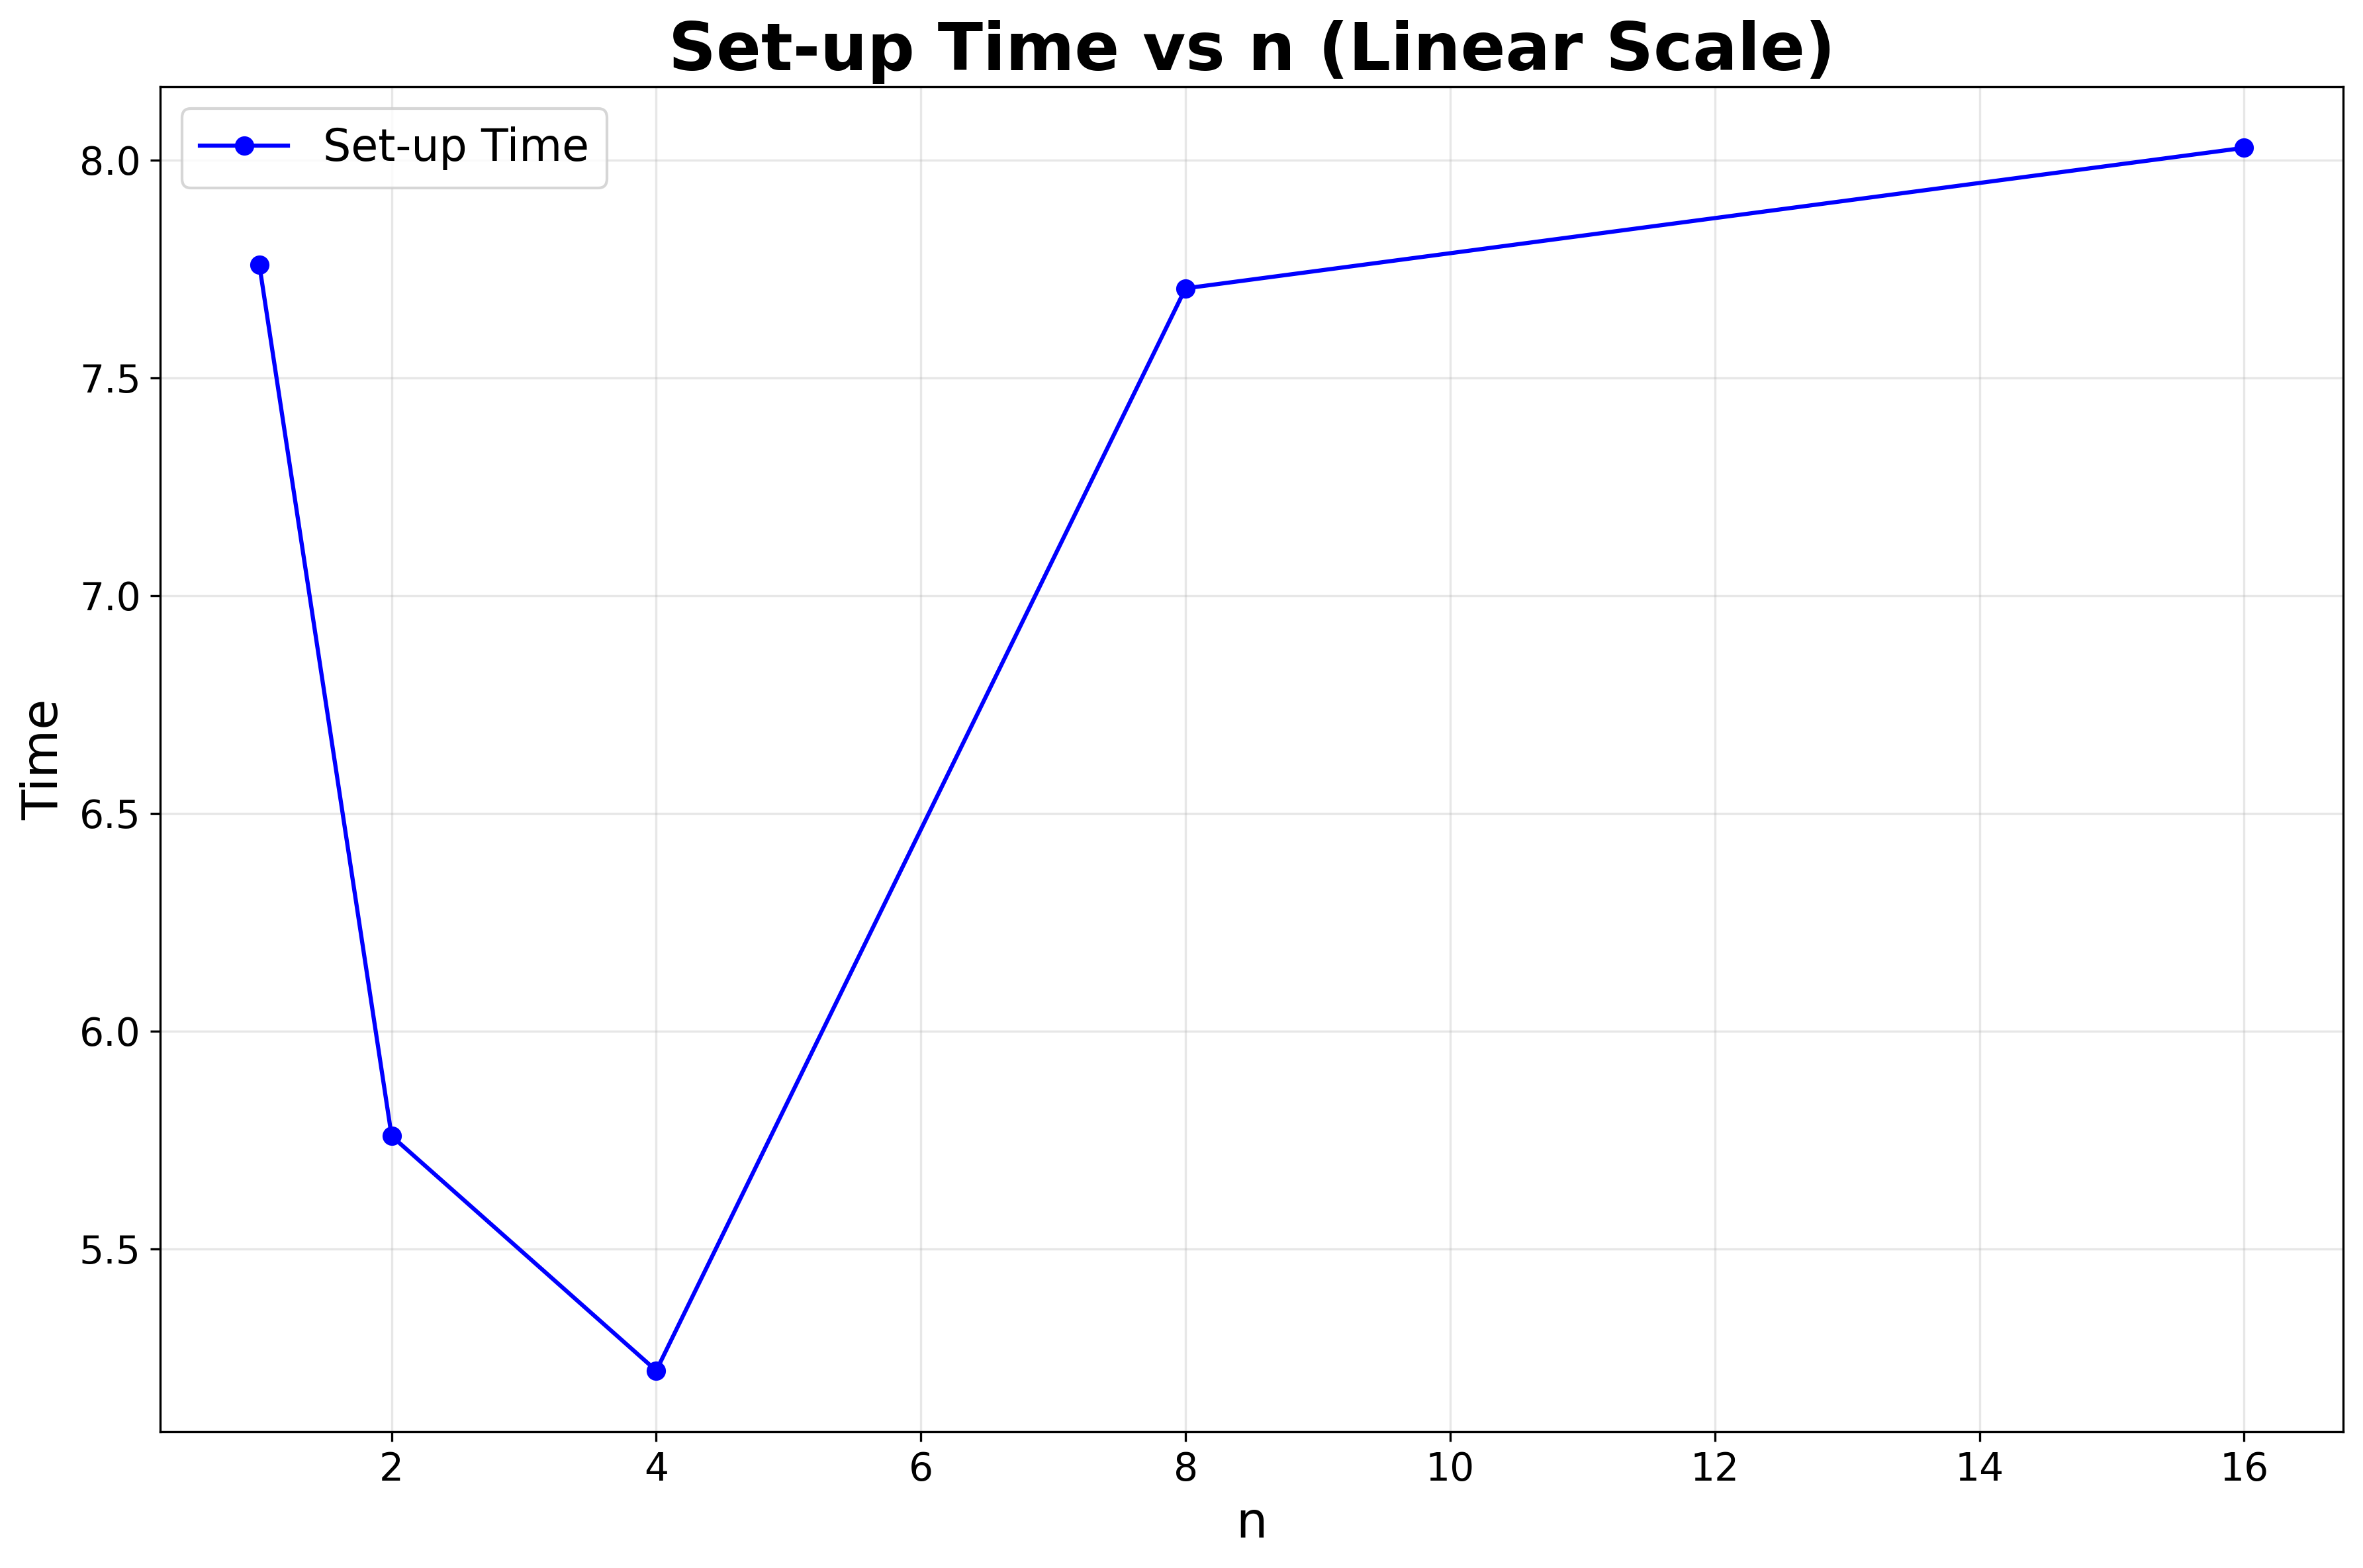
\includegraphics[width=0.7\textwidth]{img/Set-up_linear_graph.png}
  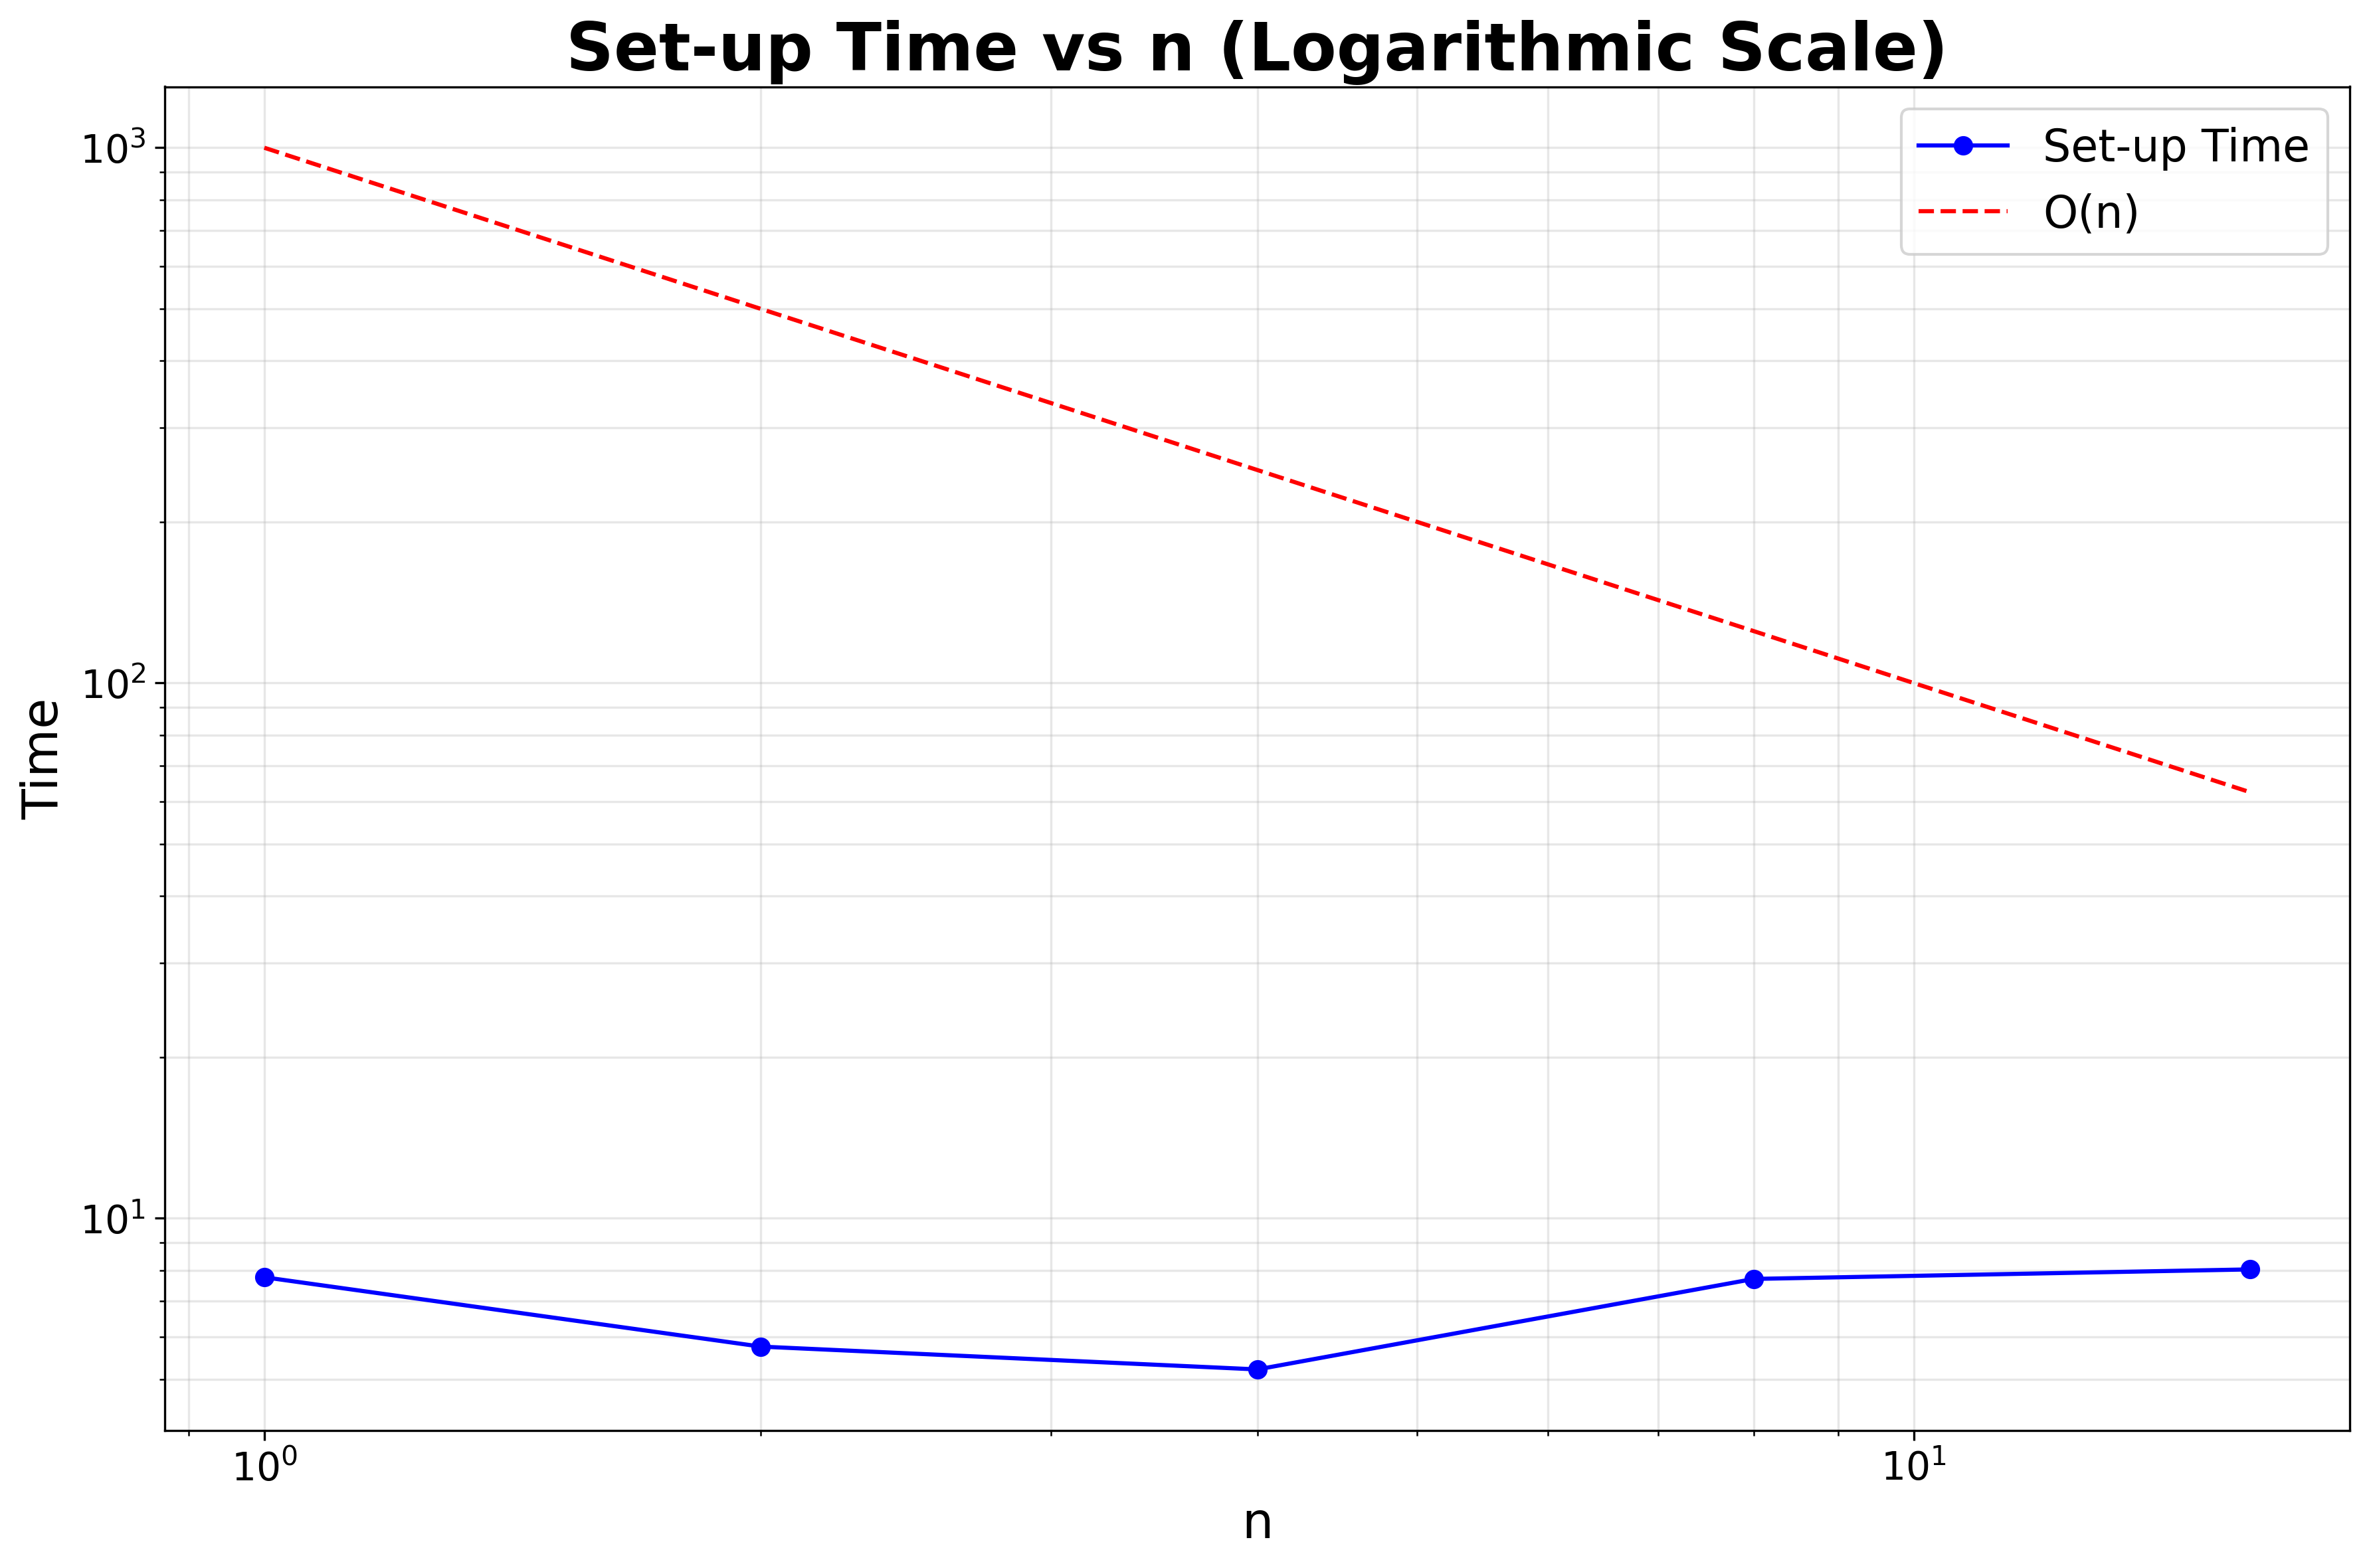
\includegraphics[width=0.7\textwidth]{img/Set-up_log_graph.png}
  \caption{Setup time of the program as a function of the number of processes. The top figure is linear scale, the bottom figure is log–log scale.}
  \label{fig:setup_time}
\end{figure}

\autoref{fig:setup_time} shows the setup time of the program with respect to the number of processes used. The setup time decreases until four processes are employed, after which it starts to increase. This behavior is caused by the communication overhead inherent in the setup phase; as the number of processes increases, the cost of inter-process communication outweighs the benefits of parallelization.

\subsection{Solve Time}
\begin{figure}[h!]
  \centering
  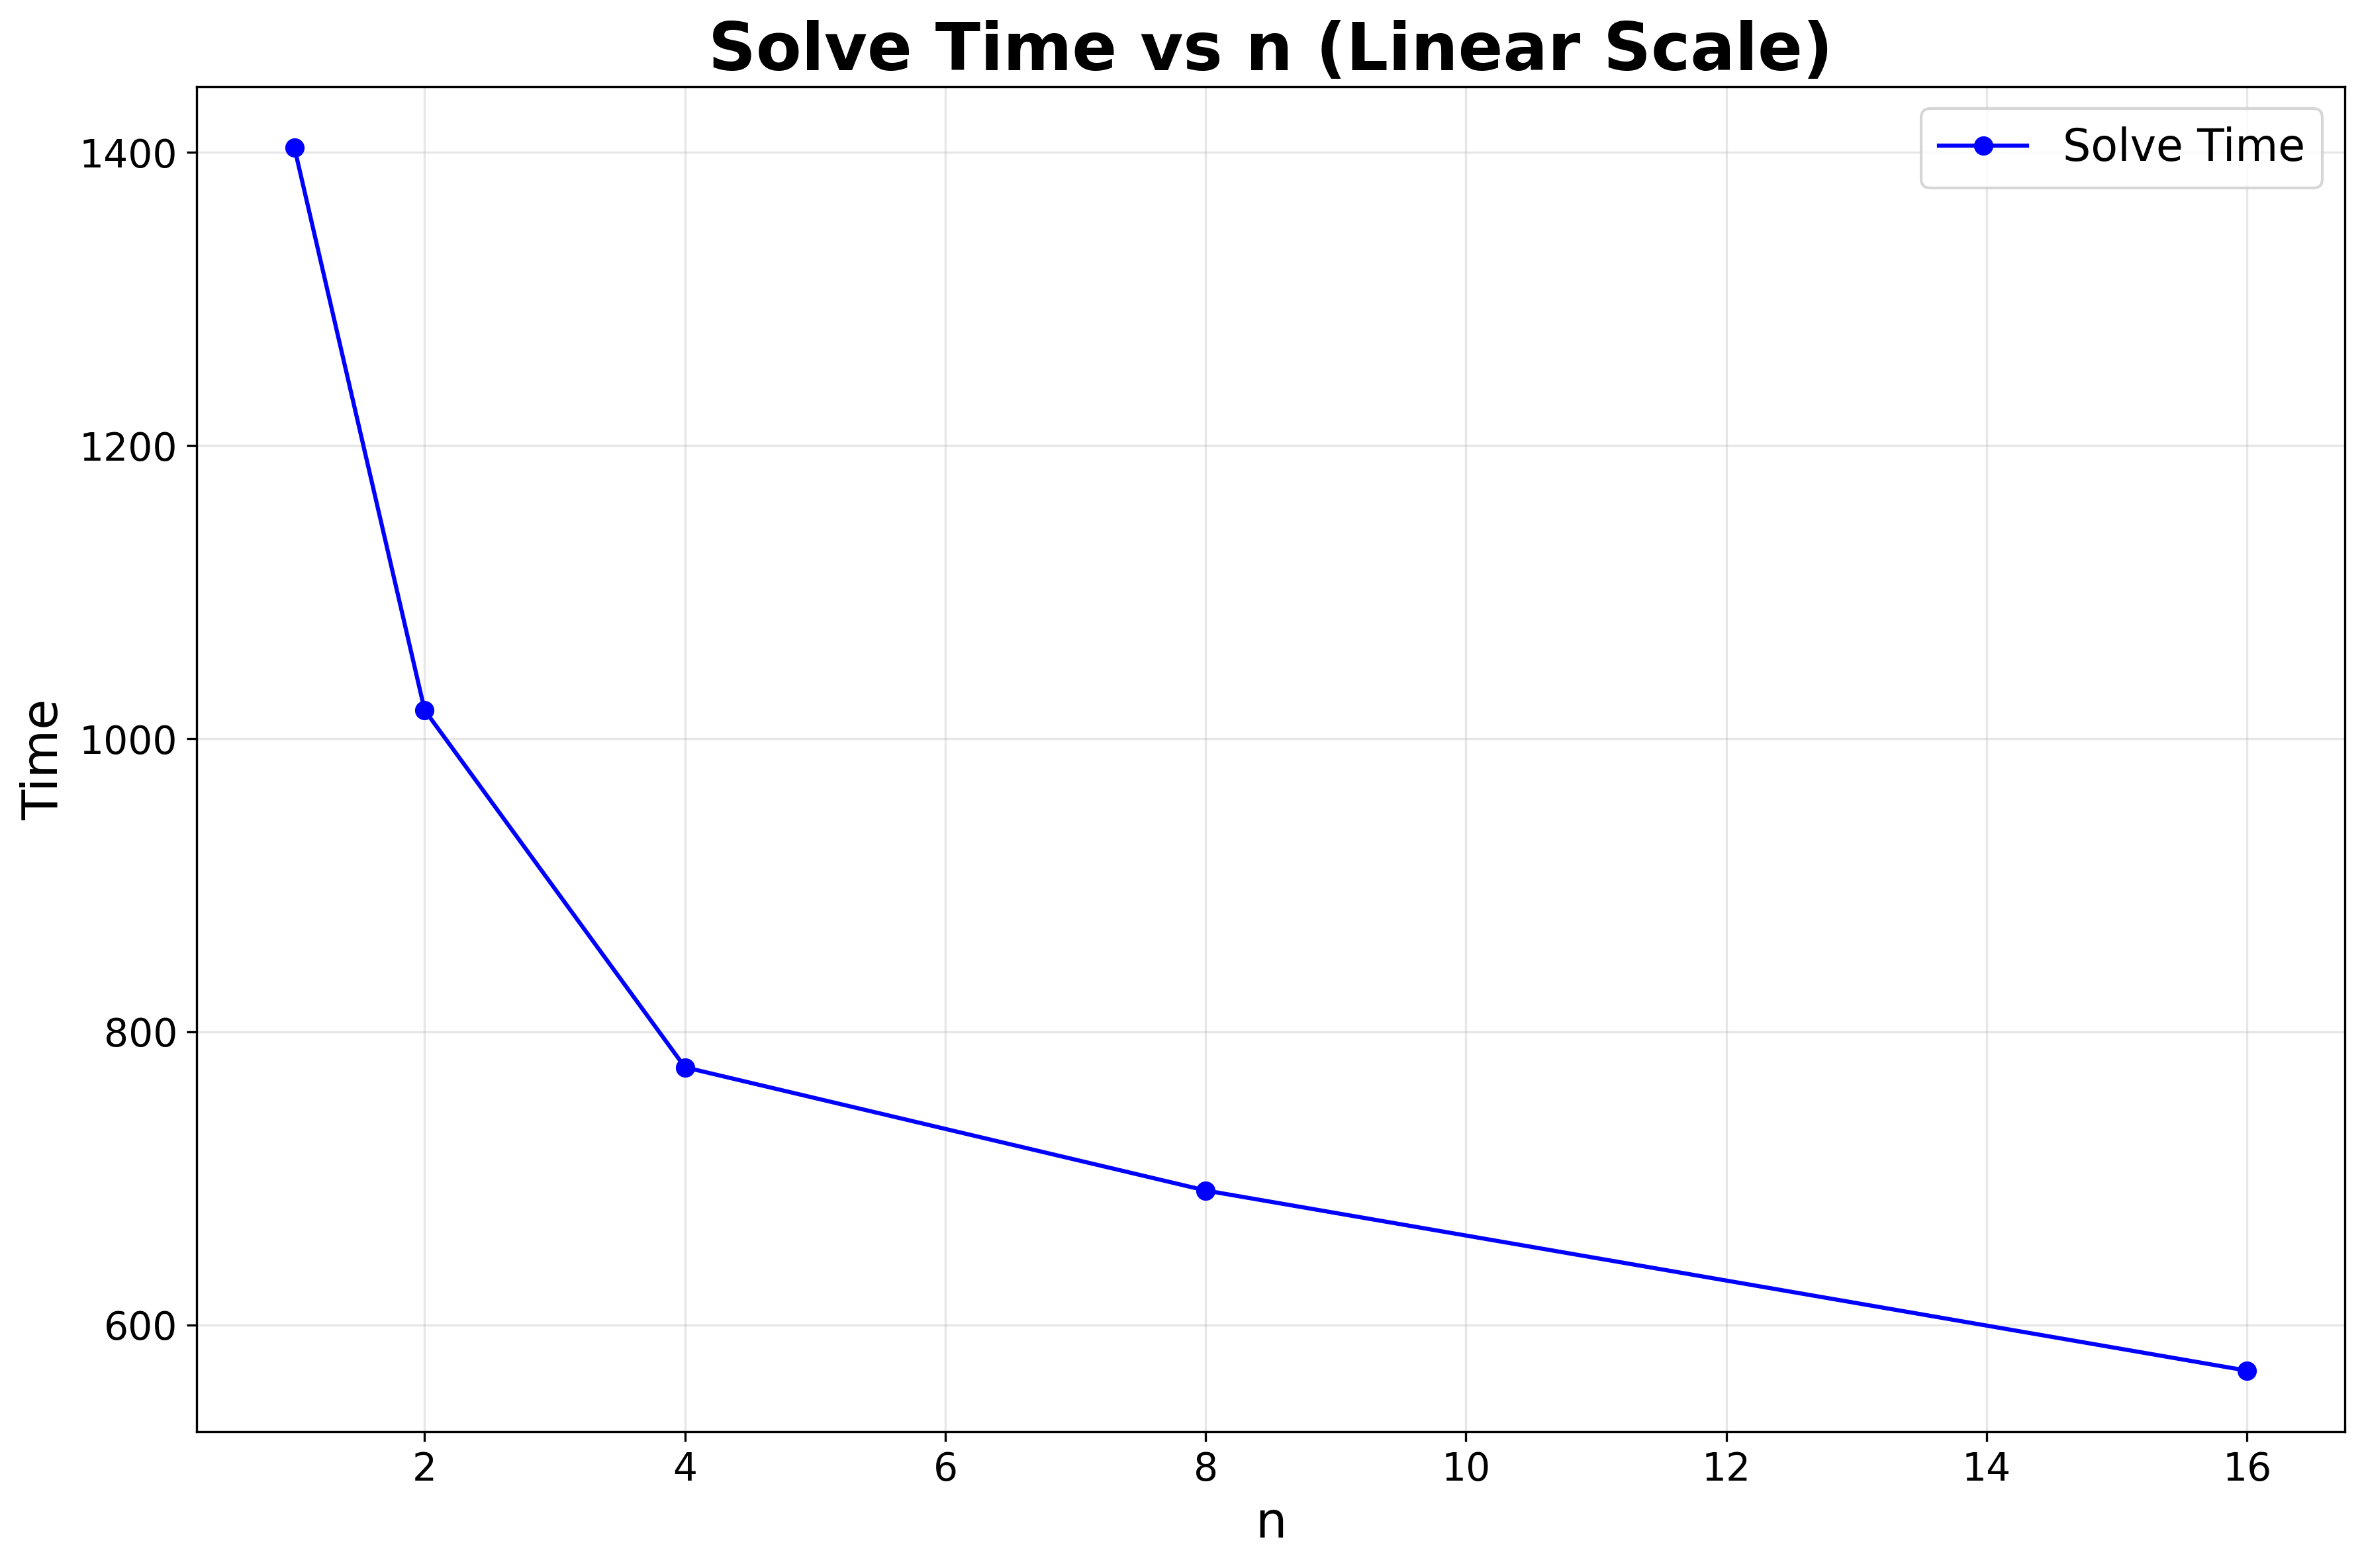
\includegraphics[width=0.7\textwidth]{img/Solve_linear_graph.png}
  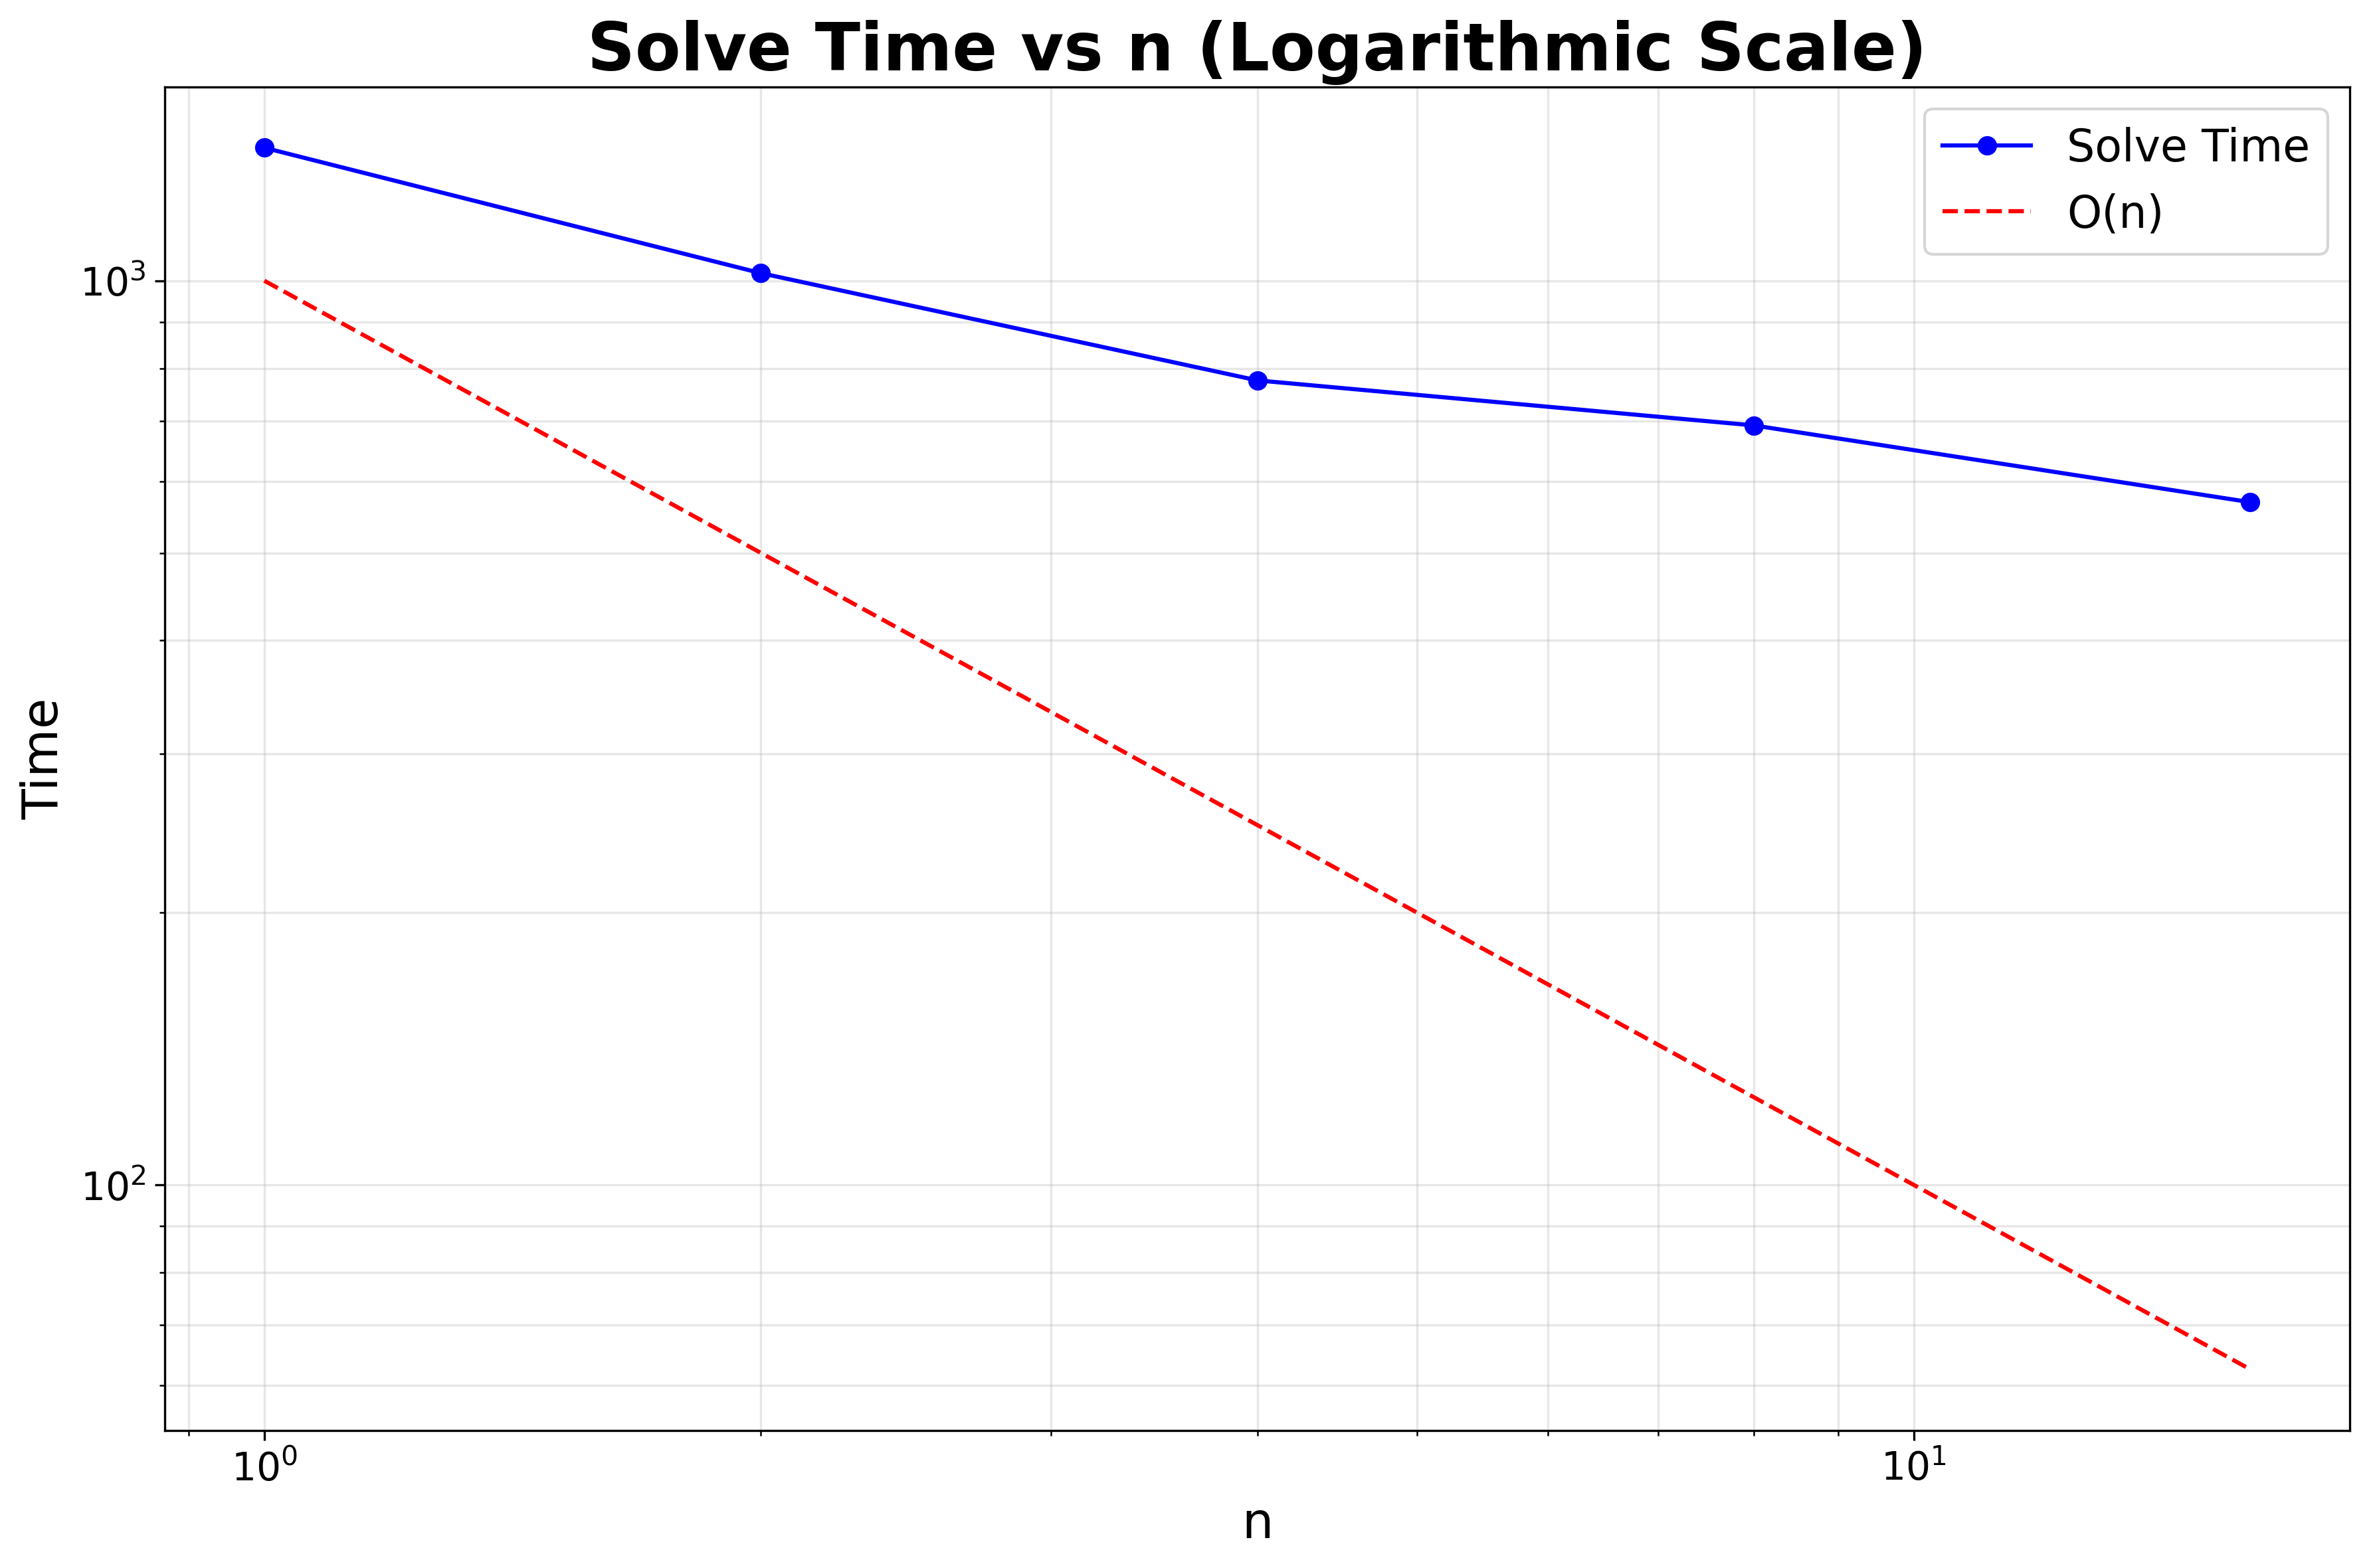
\includegraphics[width=0.7\textwidth]{img/Solve_log_graph.png}
  \caption{Solve time of the program as a function of the number of processes. The top figure is linear scale, the bottom figure is log–log scale.}
  \label{fig:solve_time}
\end{figure}

\autoref{fig:solve_time} shows the time required to solve the problem as a function of the number of processes. The solve time decreases as the number of processes increases, but the reduction is not linear. This is due to the fact that parts of the algorithm, such as the assembly of the system matrices and the Newton iterations, are inherently sequential or require synchronization between processes. As a result, the efficiency of parallelization diminishes beyond four processes, and the solve time begins to saturate.

\subsection{Total Time}
\begin{figure}[h!]
  \centering
  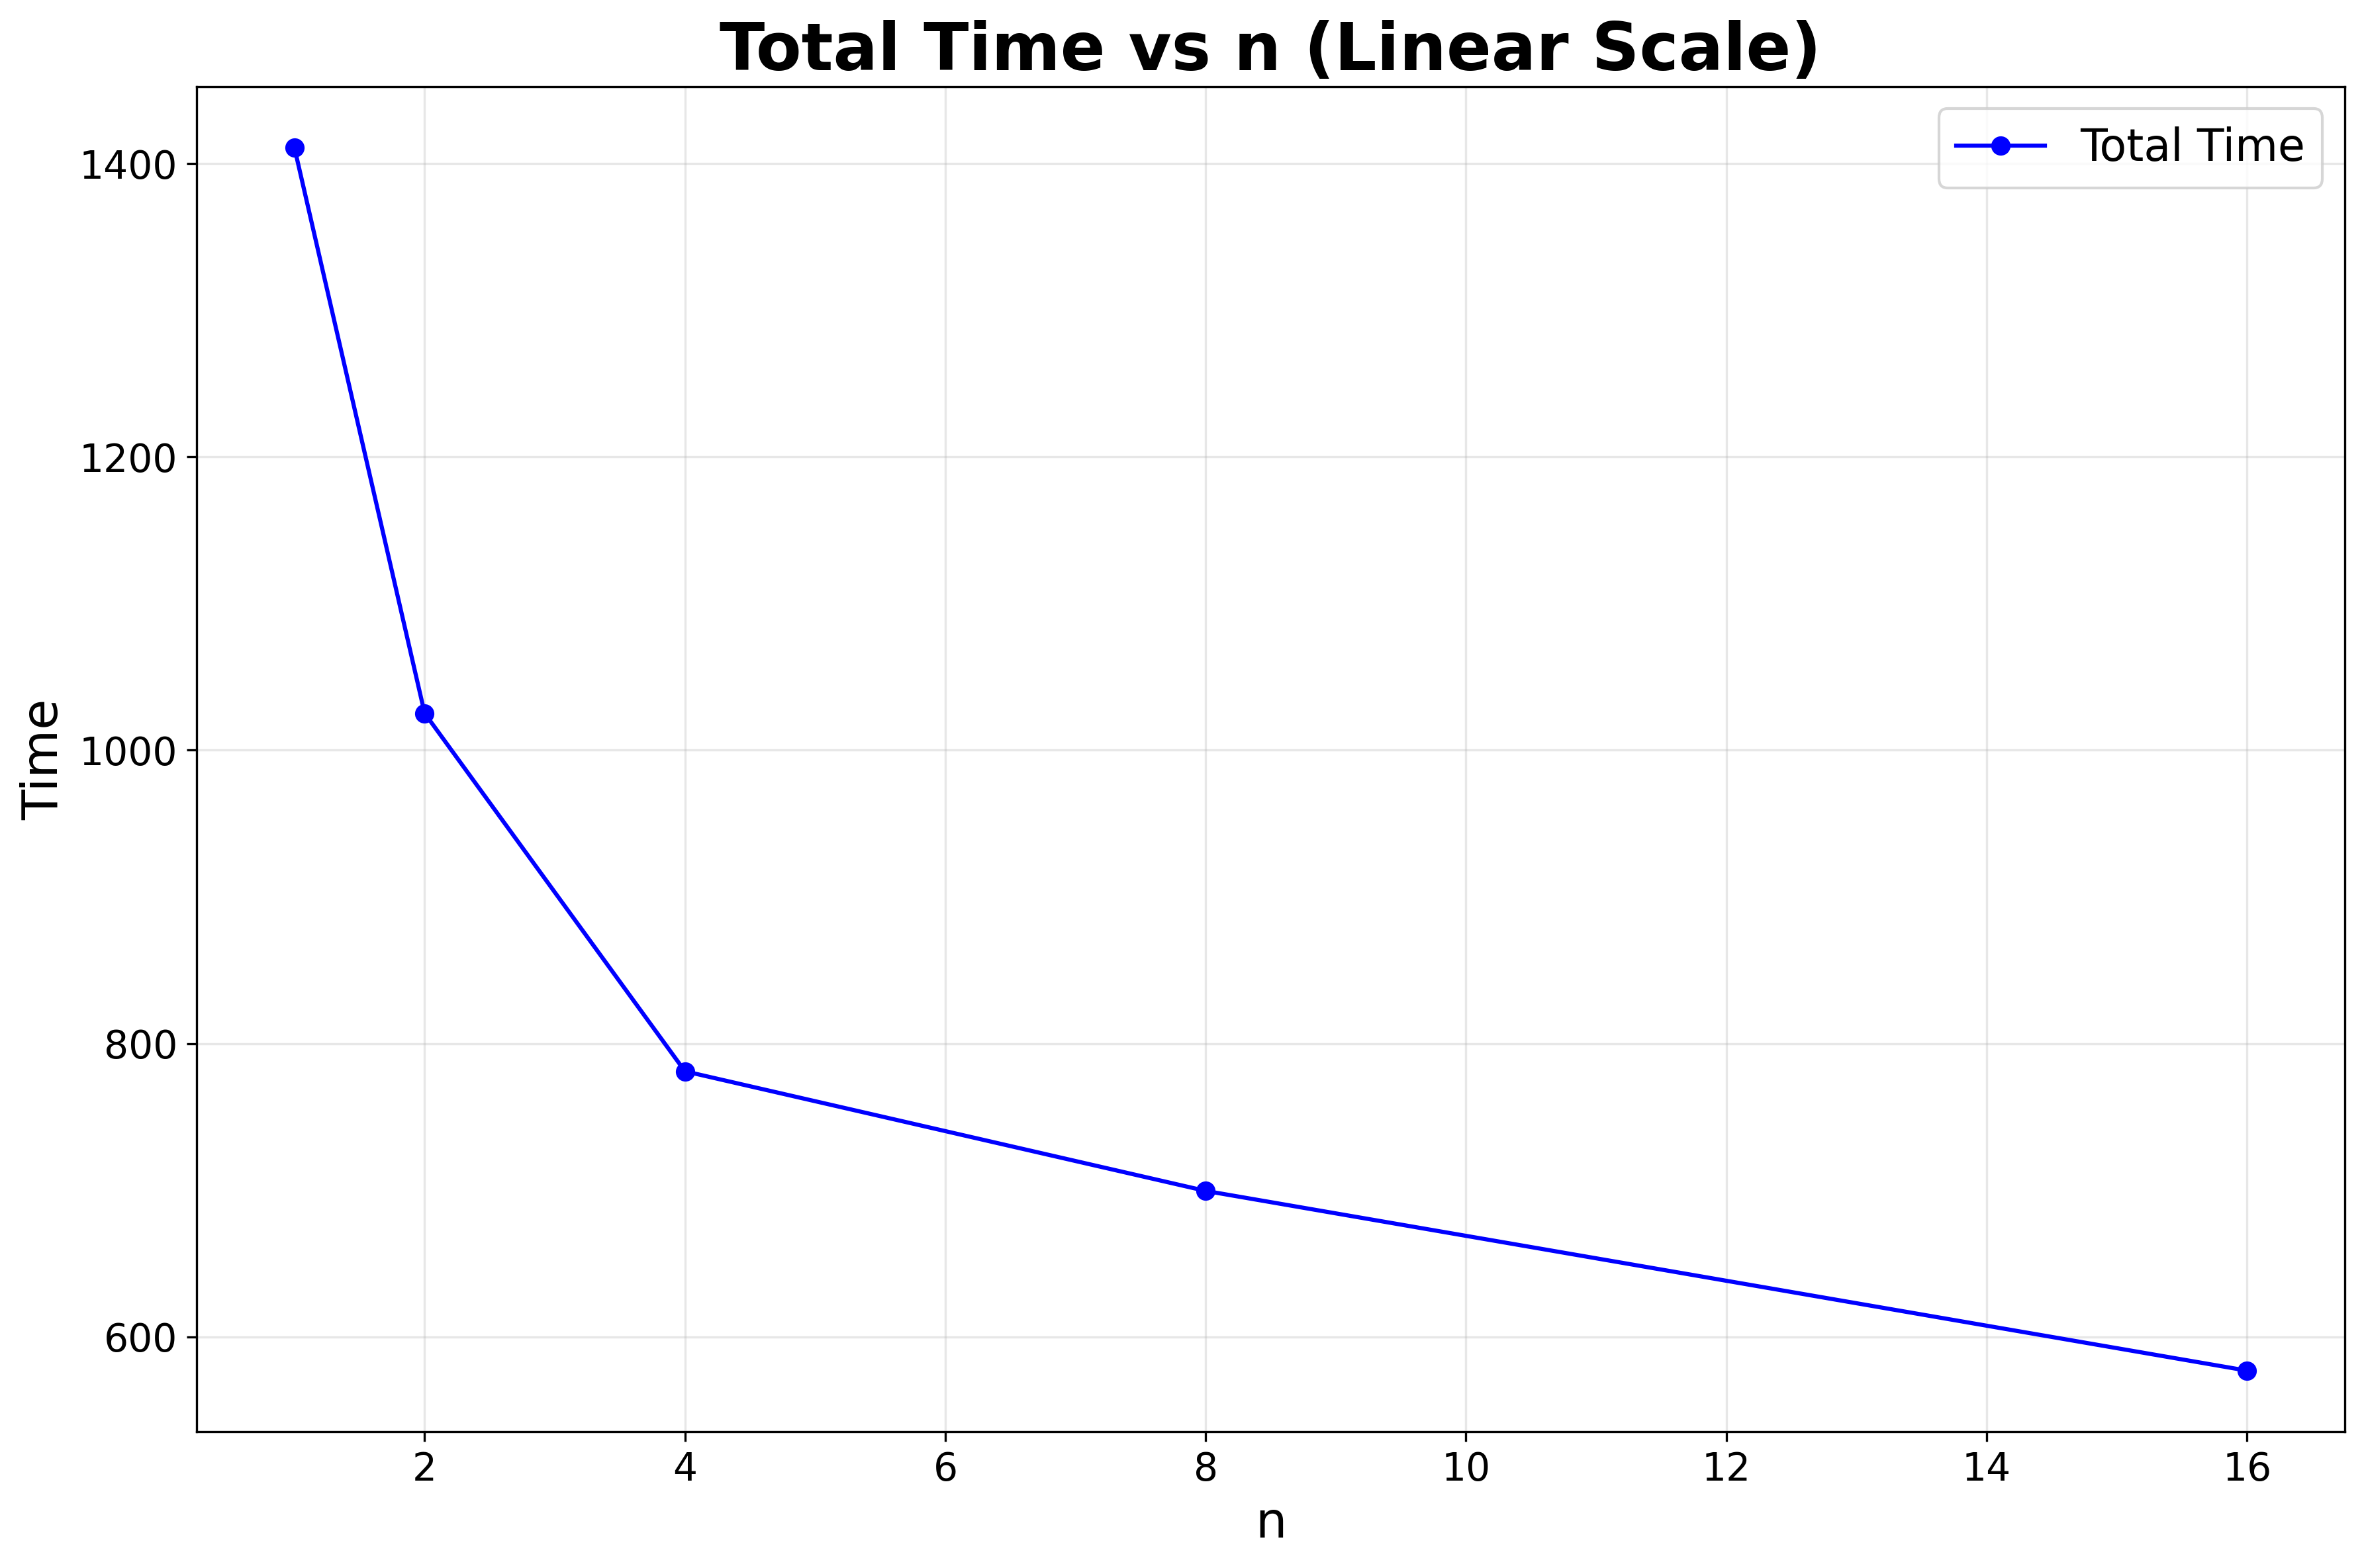
\includegraphics[width=0.7\textwidth]{img/Total_linear_graph.png}
  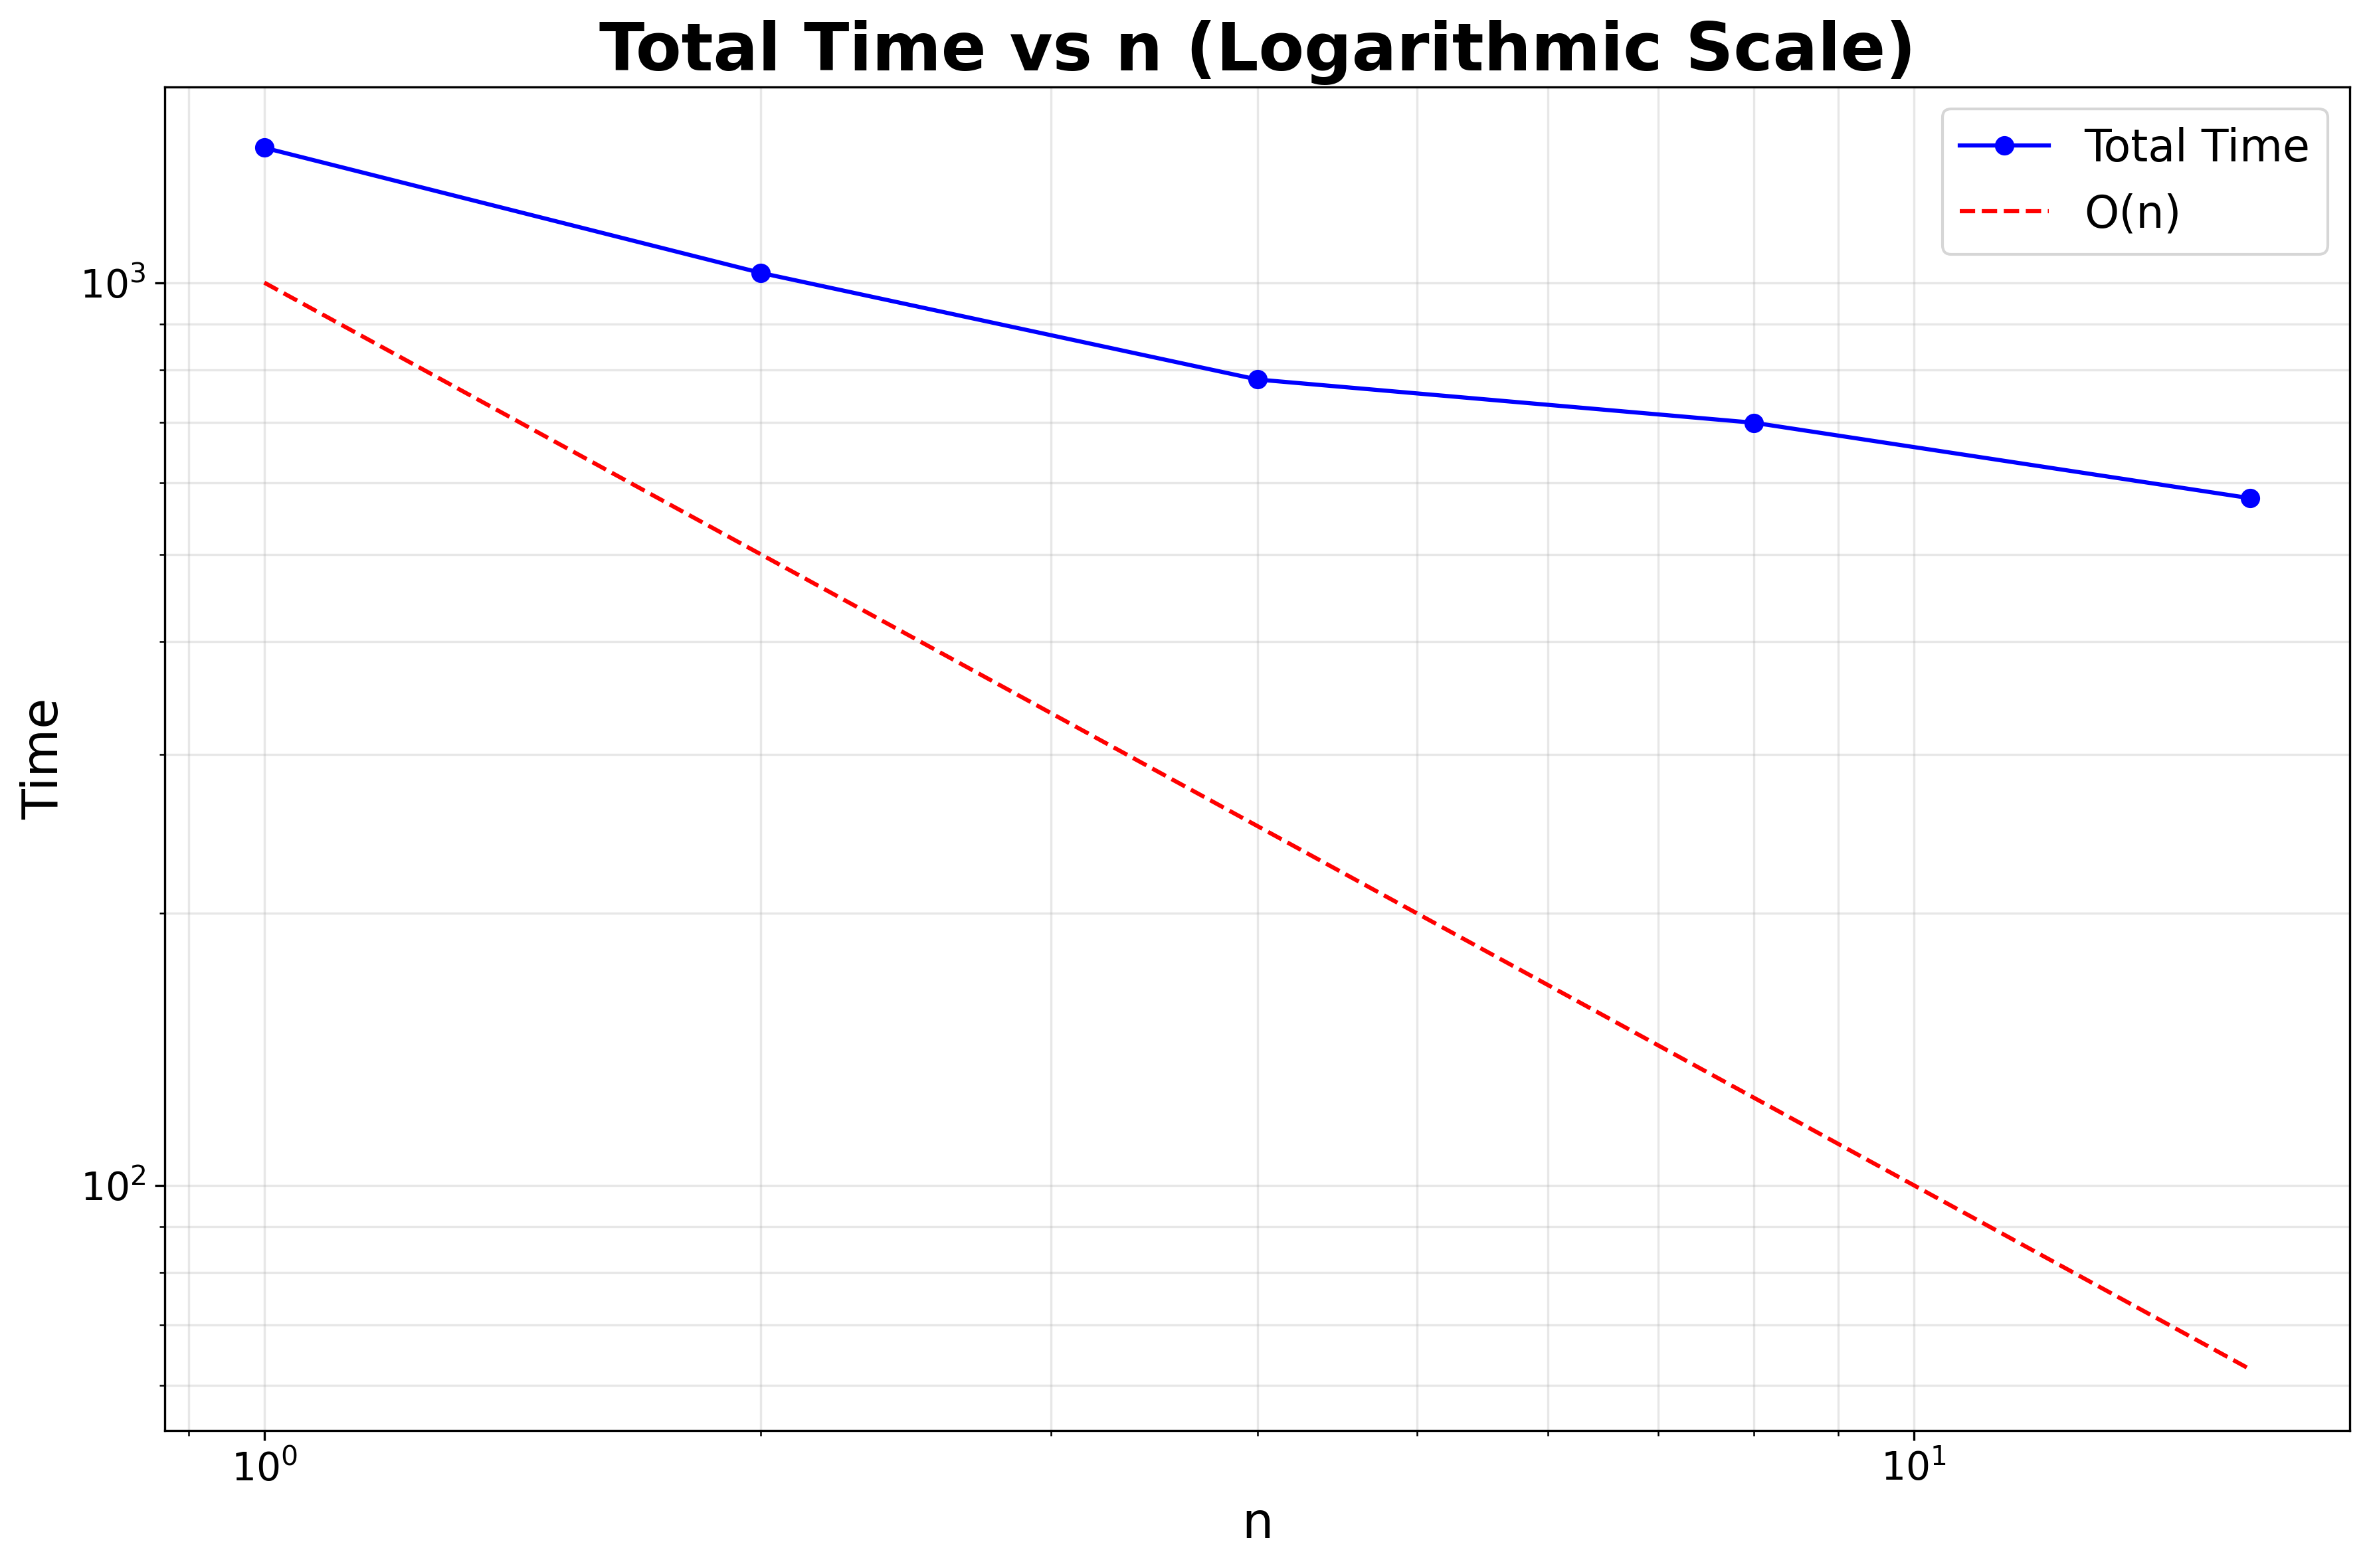
\includegraphics[width=0.7\textwidth]{img/Total_log_graph.png}
  \caption{Total runtime of the program as a function of the number of processes. The top figure is linear scale, the bottom figure is log–log scale.}
  \label{fig:total_time}
\end{figure}

\autoref{fig:total_time} reports the total runtime, which includes both setup and solve phases. As expected, the total time decreases with an increasing number of processes, but the improvement is not linear. Beyond four processes, the benefit of adding more processes is minimal.


\section{Different parameters}
We also tested the program with different parameters, in particular we used the second case of parameters from the paper, so with:
\begin{itemize}
  \item \( T = 20 \) years
  \item \( \Delta t = 1/6 \) years
  \item \( d^{ext} = [1.5, 1.5] cm^2/year\)
  \item \( d^{axn} = [0.0, 3.0] cm^2/year\)
  \item \( \alpha = [0.3, 0.6] /year\)
\end{itemize}
Where, again, the first component of the vectors refers to White Matter and the second to Grey Matter.

In both the two configurations, the program was able to run without any issues, and the results were consistent with the expected behavior of the model, compared to the results presented in the paper \cite{WEICKENMEIER2019264}.
\section{Stability and Convergence}

We will not analyze the stability and convergence of the whole project. However, to ensure that each step of our numerical method is well-posed, we can analyze the linearized problem solved within each Newton iteration. We will demonstrate that this linear problem has a unique solution by verifying the conditions of the Lax-Milgram theorem. This reduces the problem at each iteration to a standard elliptic problem, a topic covered in the course. Finally we also must verify the continuity of both the bilinear form $a(u,v)$ and the linear functional $F(v)$.

\subsection{Lax-Milgram Analysis for the Linearized Step}
At each time step $n+1$ and for each Newton iteration $k$, we solve for an update $\delta^{(k)} \in H^1(\Omega)$ that satisfies the linear weak formulation:
\[
  a(\delta^{(k)}, v) = F(v) \quad \forall v \in H^1(\Omega).
\]
This corresponds to the system $a(c_k^{n+1})(\delta^{(k)}, v) = -R(c_k^{n+1}, v)$. To maintain clarity in this section, we relabel the unknown update $\delta^{(k)}$ as $\delta$. The bilinear form $a(\cdot, \cdot)$ and linear functional $F(\cdot)$ are defined as:
\begin{align*}
  a(\delta, v) & = \int_{\Omega} \frac{1}{\Delta t} \delta v \, d\mathbf{x} + \int_{\Omega}   D \nabla \delta, \nabla v   \, d\mathbf{x} - \int_{\Omega} \alpha (1 - 2 c_k^{(n+1)}) \delta v \, d\mathbf{x},                      \\
  F(v)         & = -\int_{\Omega} \frac{c_k^{(n+1)} - c^n}{\Delta t} v \cdot d\mathbf{x} - \int_{\Omega}   D \nabla c_k^{(n+1)}, \nabla v   \, d\mathbf{x} + \int_{\Omega} \alpha c_k^{(n+1)} (1 - c_k^{(n+1)}) v \, d\mathbf{x}.
\end{align*}

\subsubsection{Assumptions}
The analysis relies on the following reasonable assumptions:
\begin{itemize}
  \item \textbf{Function Space:} The solution and test functions belong to $V = H^1(\Omega)$, with the norm $\|v\|_{H^1}^2 = \|v\|_{L^2}^2 + \|\nabla v\|_{L^2}^2$.
  \item \textbf{Diffusion Tensor:} The tensor $D = d^{\text{ext}} \mathbf{I} + d^{\text{axn}} \mathbf{n} \otimes \mathbf{n}$ is symmetric and positive definite. We assume $d^{\text{ext}}, d^{\text{axn}} \ge 0$.
  \item \textbf{Stability Assumption:} The numerical method is assumed to be stable up to the current state, implying that concentrations remain physical, i.e., $c^n, c_k^{(n+1)} \in [0, 1]$ in $\Omega$.
\end{itemize}
To apply the Lax-Milgram theorem, we must show that $a(\cdot, \cdot)$ is coercive and continuous on $H^1(\Omega)$.

\subsubsection{Coercivity of the Bilinear Form $a(\delta, v)$}

We must show that there exists a constant $\alpha_0 > 0$ such that 
\[
a(v,v) \ge \alpha_0 \norm{v}_{H^1(\Omega)}^2 \quad \forall v \in H^1(\Omega).
\]

Using the definition of the bilinear form, we have
\begin{align*}
  a(v,v) 
  &= \int_{\Omega} \frac{1}{\Delta t} v^2 \, \dd \vb{x} + \int_{\Omega} \vb{\nabla} v \cdot D \, \vb{\nabla} v \, \dd \vb{x} - \int_{\Omega} \alpha \left(1 - 2c_k^{n+1}\right) v^2 \, \dd \vb{x} \\
  &= \int_{\Omega} \left( \frac{1}{\Delta t} - \alpha \left(1 - 2c_k^{n+1}\right) \right) v^2 \, \dd \vb{x} 
     + \int_{\Omega} \vb{\nabla} v \cdot \left( d^{\mathrm{ext}} \mathbf{I} + d^{\mathrm{axn}} \, \vb{n} \otimes \vb{n} \right) \vb{\nabla} v \, \dd \vb{x} \\
  &= \int_{\Omega} \left( \frac{1}{\Delta t} - \alpha \left(1 - 2c_k^{n+1}\right) \right) v^2 \, \dd \vb{x} 
     + \int_{\Omega} d^{\mathrm{ext}} \norm{\vb{\nabla} v}^2 \, \dd \vb{x} 
     + \int_{\Omega} d^{\mathrm{axn}} \left( \vb{n} \cdot \vb{\nabla} v \right)^2 \, \dd \vb{x}.
\end{align*}

Since $d^{\mathrm{axn}} \ge 0$, the last term is non-negative. Therefore, we can establish the lower bound
\[
a(v,v) \ge M \norm{v}_{L^2(\Omega)}^2 + N \norm{\vb{\nabla} v}_{L^2(\Omega)}^2,
\]
where the constants $M$ and $N$ are defined as the essential infima over the domain:
\[
M := \essinf_{\vb{x} \in \Omega} \left( \frac{1}{\Delta t} - \alpha \left(1 - 2c_k^{n+1}\right) \right), 
\quad 
N := \essinf_{\vb{x} \in \Omega} d^{\mathrm{ext}}.
\]

For coercivity, it is required that $M > 0$ and $N > 0$. In this case, we can set $\alpha_0 = \min(M, N) > 0$, which implies
\[
a(v,v) \ge M \norm{v}_{L^2(\Omega)}^2 + N \norm{\vb{\nabla} v}_{L^2(\Omega)}^2 \ge \alpha_0 \norm{v}_{H^1(\Omega)}^2.
\]

This leads to two conditions for well-posedness at each Newton step:
\begin{enumerate}
  \item $\essinf_{\vb{x} \in \Omega} d^{\mathrm{ext}} > 0$, i.e., the diffusion is non-degenerate.
  \item $\dfrac{1}{\Delta t} > \esssup_{\vb{x} \in \Omega} \alpha \left(1 - 2 c_k^{n+1}\right) = \norm{\alpha (1 - 2 c_k^{n+1})}_{L^\infty(\Omega)}$.
\end{enumerate}


\subsection{Continuity of the Bilinear Form $a(u, v)$}

The bilinear form arises from the left-hand side of the linearized weak formulation and is defined as
\[
a(u, v) = \int_{\Omega} \frac{u v}{\Delta t} \, \dd \vb{x} + \int_{\Omega} \vb{\nabla} u \cdot D \, \vb{\nabla} v \, \dd \vb{x} - \int_{\Omega} \alpha \left(1 - 2 c_k^{n+1}\right) u v \, \dd \vb{x},
\]
where the diffusion tensor is 
\[
D = d^{\mathrm{ext}} \mathbf{I} + d^{\mathrm{axn}} \, \vb{n} \otimes \vb{n}.
\]

We aim to show that there exists a constant $M > 0$ such that
\[
\abs{a(u, v)} \le M \, \norm{u}_{V} \norm{v}_{V} \quad \forall u, v \in V,
\]
where $V$ is the appropriate Hilbert space (e.g., $H^1(\Omega)$). We analyze the form term by term using the triangle inequality:
\begin{align*}
\abs{a(u, v)} &\le 
\left| \int_{\Omega} \left( \frac{1}{\Delta t} - \alpha \left(1-2c_k^{n+1}\right) \right) u v \, \dd \vb{x} \right| \\
&\quad + \left| \int_{\Omega} d^{\mathrm{ext}} \vb{\nabla} u \cdot \vb{\nabla} v \, \dd \vb{x} \right| \\
&\quad + \left| \int_{\Omega} d^{\mathrm{axn}} \left( \vb{n} \cdot \vb{\nabla} u \right) \left( \vb{n} \cdot \vb{\nabla} v \right) \, \dd \vb{x} \right|.
\end{align*}

\paragraph{1. Time Derivative and Reaction Term} 
We bound the first term using the Cauchy-Schwarz and Poincaré inequalities:
\begin{align*}
\abs{\int_{\Omega} \left( \frac{1}{\Delta t} - \alpha(1-2c_k^{n+1}) \right) u v \, \dd \vb{x}}
& \le \norm{\frac{1}{\Delta t} - \alpha (1-2c_k^{n+1})}_{L^\infty} \int_{\Omega} \abs{u v} \, \dd \vb{x} \\
& \le \norm{\frac{1}{\Delta t} - \alpha (1-2c_k^{n+1})}_{L^\infty} \, \norm{u}_{L^2} \, \norm{v}_{L^2} \\
& \le C_P \left( \frac{1}{\Delta t} + \norm{\alpha (1-2c_k^{n+1})}_{L^\infty} \right) \norm{u}_{V} \norm{v}_{V},
\end{align*}
where $C_P$ is the Poincaré constant.

\paragraph{2. Isotropic Diffusion Term} 
The isotropic diffusion term is bounded by Cauchy-Schwarz:
\[
\abs{\int_{\Omega} d^{\mathrm{ext}} \vb{\nabla} u \cdot \vb{\nabla} v \, \dd \vb{x}} \le \norm{d^{\mathrm{ext}}}_{L^\infty} \, \norm{\vb{\nabla} u}_{L^2} \, \norm{\vb{\nabla} v}_{L^2}.
\]

\paragraph{3. Anisotropic Diffusion Term} 
For the anisotropic term, since $\vb{n}$ is a unit vector field ($\norm{\vb{n}}_{L^\infty} = 1$), we have
\begin{align*}
\abs{\int_{\Omega} d^{\mathrm{axn}} (\vb{n} \cdot \vb{\nabla} u)(\vb{n} \cdot \vb{\nabla} v) \, \dd \vb{x}}
& \le \norm{d^{\mathrm{axn}}}_{L^\infty} \int_{\Omega} \abs{\vb{n} \cdot \vb{\nabla} u} \, \abs{\vb{n} \cdot \vb{\nabla} v} \, \dd \vb{x} \\
& \le \norm{d^{\mathrm{axn}}}_{L^\infty} \, \norm{\vb{n} \cdot \vb{\nabla} u}_{L^2} \, \norm{\vb{n} \cdot \vb{\nabla} v}_{L^2} \\
& \le \norm{d^{\mathrm{axn}}}_{L^\infty} \, \norm{\vb{\nabla} u}_{L^2} \, \norm{\vb{\nabla} v}_{L^2}.
\end{align*}

By combining these bounds, we conclude that the bilinear form $a(u,v)$ is continuous, provided that the concentration $c_k^{n+1}$ is bounded in $L^\infty(\Omega)$ at each iteration, which is physically reasonable since $c$ represents a normalized concentration.

\subsection{Continuity of the Linear Functional $F(v)$}

The linear functional $F(v)$ represents the residual from the right-hand side of the linearized system:
\[
F(v) = - \int_{\Omega} \frac{c_k^{n+1} - c^n}{\Delta t} \, v \, \dd \vb{x} 
       - \int_{\Omega} \vb{\nabla} c_k^{n+1} \cdot D \, \vb{\nabla} v \, \dd \vb{x} 
       + \int_{\Omega} \alpha \, c_k^{n+1} \left(1 - c_k^{n+1}\right) v \, \dd \vb{x},
\]
where the diffusion tensor is
\[
D = d^{\mathrm{ext}} \mathbf{I} + d^{\mathrm{axn}} \, \vb{n} \otimes \vb{n}.
\]

We want to show that there exists a constant $\bar{K} > 0$ such that
\[
\abs{F(v)} \le \bar{K} \, \norm{v}_V \quad \forall v \in V,
\]
where $V$ is the appropriate Hilbert space (e.g., $H^1(\Omega)$). Using the triangle inequality, we split $F(v)$ into terms without and with gradients of $v$:
\[
\abs{F(v)} \le 
\abs{\int_{\Omega} \left( \alpha \, c_k^{n+1}(1 - c_k^{n+1}) - \frac{c_k^{n+1} - c^n}{\Delta t} \right) v \, \dd \vb{x}}
+
\abs{\int_{\Omega} \vb{\nabla} c_k^{n+1} \cdot D \, \vb{\nabla} v \, \dd \vb{x}}.
\]

\paragraph{1. Terms without Gradient of $v$} 
This term combines the reaction and time-stepping contributions. Using the Cauchy-Schwarz and Poincaré inequalities:
\begin{align*}
& \abs{\int_{\Omega} \left( \alpha \, c_k^{n+1}(1 - c_k^{n+1}) - \frac{c_k^{n+1} - c^n}{\Delta t} \right) v \, \dd \vb{x}} \\
&\quad \le \left( \norm{\alpha \, c_k^{n+1}(1 - c_k^{n+1})}_{L^\infty} + \norm{\frac{c_k^{n+1} - c^n}{\Delta t}}_{L^\infty} \right) \int_{\Omega} \abs{v} \, \dd \vb{x} \\
&\quad \le C \left( \norm{\alpha \, c_k^{n+1}(1 - c_k^{n+1})}_{L^\infty} + \norm{\frac{c_k^{n+1} - c^n}{\Delta t}}_{L^\infty} \right) \norm{v}_{L^2} \\
&\quad \le C' \norm{v}_V,
\end{align*}
where $C'$ depends on the Poincaré constant and the domain volume.

\paragraph{2. Terms with Gradient of $v$} 
This term arises from the diffusion operator. Splitting into isotropic and anisotropic contributions and applying Cauchy-Schwarz:
\begin{align*}
& \abs{\int_{\Omega} \vb{\nabla} c_k^{n+1} \cdot D \, \vb{\nabla} v \, \dd \vb{x}} \\
&\quad \le \abs{\int_{\Omega} d^{\mathrm{ext}} \, \vb{\nabla} c_k^{n+1} \cdot \vb{\nabla} v \, \dd \vb{x}} 
       + \abs{\int_{\Omega} d^{\mathrm{axn}} (\vb{n} \cdot \vb{\nabla} c_k^{n+1})(\vb{n} \cdot \vb{\nabla} v) \, \dd \vb{x}} \\
&\quad \le \left( \norm{d^{\mathrm{ext}}}_{L^\infty} + \norm{d^{\mathrm{axn}}}_{L^\infty} \right) \norm{\vb{\nabla} c_k^{n+1}}_{L^2} \norm{\vb{\nabla} v}_{L^2}.
\end{align*}

\paragraph{Conclusion} 
Combining the above bounds, we obtain
\[
\abs{F(v)} \le 
\left[ C' + \left( \norm{d^{\mathrm{ext}}}_{L^\infty} + \norm{d^{\mathrm{axn}}}_{L^\infty} \right) \norm{\vb{\nabla} c_k^{n+1}}_{L^2} \right] \norm{v}_V.
\]
Thus, the linear functional $F(v)$ is continuous, provided the following quantities remain bounded during the iterative process:
\begin{itemize}
  \item $\norm{c_k^{n+1} - c^n}_{L^\infty}$,
  \item $\norm{\alpha \, c_k^{n+1} (1 - c_k^{n+1})}_{L^\infty}$,
  \item $\norm{\vb{\nabla} c_k^{n+1}}_{L^2}$.
\end{itemize}
These conditions are physically and mathematically reasonable for a well-behaved solution over a finite domain.

\subsubsection{Summary of Conditions}
The Lax-Milgram theorem guarantees a unique solution for the linear system at each Newton step if the problem data and numerical solution satisfy certain criteria.

\paragraph{Assumptions on Problem Data (assumed to hold):}
\begin{itemize}
  \item The diffusion coefficients and reaction parameter are bounded:

        $\|D_{\text{iso}}\|_{L^\infty}, \|D_{\text{aniso}}\|_{L^\infty}, \|\alpha\|_{L^\infty} < \infty$.
  \item The isotropic part of the diffusion is non-degenerate:

        $\underset{\Omega}{\operatorname{ess\,inf}} \, D_{\text{iso}} > 0$.
\end{itemize}

\paragraph{Assumptions on the Numerical Solution (related to stability):}
\begin{itemize}
  \item Concentrations are bounded: $c^n, c_k^{n+1} \in [0,1]$.
  \item The previous iterate is sufficiently regular: $\|c_k^{n+1}\|_{H^1} < \infty$.
\end{itemize}

\paragraph{Critical Condition for Coercivity and Convergence:}
Given the assumptions above, the crucial condition that must be satisfied for the problem to be well-posed is the time step restriction:
\[
  \frac{1}{\Delta t} > \|\alpha \cdot \left(1 - 2c_k^{n+1}\right)\|_{L^\infty}.
\]
Since our stability assumption implies $c_k^{n+1} \in [0,1]$, we have $|1-2c_k^{n+1}| \le 1$. Therefore, a sufficient condition is $\frac{1}{\Delta t} > \|\alpha\|_{L^\infty}$. This highlights the critical trade-off: a large reaction rate $\alpha$ requires a small time step $\Delta t$ to ensure the coercivity of the system matrix. If this inequality is violated, the bilinear form may cease to be coercive, leading to the divergence of the Newton iteration and failure of the simulation.
To check whether our result holds in practice, we tried to run our code with the following parameters:
\begin{itemize}
  \item \( T = 40 \) years
  \item \( \Delta t = 0.5 \) years
  \item \( d^{ext} = [6.0, 6.0] cm^2/year\)
  \item \( d^{axn} = [3.0, 3.0] cm^2/year\)
  \item \( \alpha = [3.0, 3.0] /year\)
\end{itemize}.

With these parameters we found out that the simulation doesn't converge, since the coercivity condition
\[
  \frac{1}{\Delta t} > \|\alpha\|_{L^\infty}
\]
was violated (here $1/\Delta t = 2 < \|\alpha\|_\infty = 3$). As a result, the bilinear form lost coercivity, the system matrix became indefinite, and the Newton iteration diverged already after the first step.

\chapter{Conclusion}
As a first thing, we would like to properly thank with our best regards Professor Johannes Weickenmeier, co-author of the paper used for this work, that kindly provided the original mesh used for the paper.

In this project, we have implemented a numerical model to simulate the prion-like propagation of misfolded proteins, a key mechanism in neurodegenerative diseases. By adopting the Fisher-Kolmogorov equation, we modelled the essential dynamics of protein aggregation and diffusion through a nonlinear reaction-diffusion framework. The methodology—involving a weak formulation, the unconditionally stable Backward Euler method for time discretization, and Newton-Raphson linearization—proved to be a highly effective approach reaching the same results obtained by Professor Weickenmeier in \cite{WEICKENMEIER2019264}.

Our results align with the expected behavior, demonstrating logistic growth coupled with spatial diffusion. This work serves not merely as a proof of concept but as a successful validation of the theoretical model, confirming its power to simulate complex biological phenomena.

While applied here to neurobiology, the finite element framework used in this project is a cornerstone of modern computational science with vast applicability. Reaction-diffusion systems and similar partial differential equations model phenomena across numerous fields.
This project, therefore, also serves as a manifest to the versatility of computational methods in translating mathematical models into predictive tools across diverse scientific and industrial domains.

Some ideas for expanding the capabilities of this model:

\begin{enumerate}
  \item Develop Patient-Specific Models: Integrate patient-specific brain geometries obtained from MRI scans. This would transition the model from a general representation to a potential clinical tool for personalized disease progression forecasting.
  \item Solve the Inverse Problem: Use existing clinical data to work backward and estimate key biological parameters like the local reaction rate or diffusion coefficients. This could help uncover patient-specific disease characteristics.
  \item Improve Computational Efficiency: Implement adaptive mesh refinement, where the mesh resolution increases only in areas with high activity (i.e., where the concentration gradient is steep), optimizing computational resources and enabling larger, more detailed simulations.
\end{enumerate}

\nocite{*}







\bibliographystyle{IEEEtran}
\bibliography{reference}

\end{document}